\documentclass[12pt,a4paper]{book}
\usepackage{booktabs}

\usepackage[T1]{fontenc}
%\usepackage[latin1]{inputenc} % writing of äöüß possible, instead of "a"o"u"s
\usepackage[utf8]{inputenc}
\usepackage{mathptmx} % font times-roman for math. Formulas, bullets, etc.
\usepackage{fancyhdr} % chapternames at top of page
\usepackage{longtable}
\usepackage{multicol}
\usepackage{sectsty}
\usepackage[ngerman,english]{babel}\selectlanguage{english}
\usepackage{makeidx} % allows for an index
\usepackage{subfigure} % enable subfigures
\usepackage[nottoc,notindex]{tocbibind} % include bib in toc
\usepackage[subfigure]{tocloft}
\usepackage{ifthen} % allow sophisticated control structures
\usepackage{substr} % allows substring detection

\usepackage{array}
\usepackage{colortbl}

\usepackage[top=2cm, bottom=1.25in, left=2cm, right=2cm]{geometry}
\usepackage{url}
%COLORS
\label{Color Definition}
\usepackage{xcolor}
%\definecolor{platinum}{HTML}{E5E4E2}
%\colorlet{diagrambg}{platinum}

\makeindex

\definecolor{pinkaccent}{HTML}{F50057}


\newcommand{\mytitle}{Supporting Password Coping Strategies\\with Persuasive Design}
\newcommand{\mysubtitle}{}
\newcommand{\myname}{Tobias Seitz}
\newcommand{\ie}{i.e.,\ }
\newcommand{\eg}{e.g.,\ }

\author{\myname\\\small tobias.seitz@ifi.lmu.de}
\title{\mytitle\\
\mysubtitle\\}
\date{\today}



%Stats

\newcommand{\statslt}[3]{\textit{F\textsubscript{#1}}~$=$~#2, \textit{p}~$<$~#3}
\newcommand{\stats}[3]{\textit{F\textsubscript{#1}}~$=$~#2, \textit{p}~$=$~#3}
\newcommand{\pval}[1]{\textit{p}~$=$~#1}
\newcommand{\pvallt}[1]{\textit{p}~$<$~#1}
\newcommand{\mean}[2]{\textit{m}~$=$~#1, \textit{sd}~$=$~#2}
\newcommand{\meant}[2]{\textit{m}$=$#1 \textit{sd}$=$#2}
\newcommand{\meanonly}[1]{\textit{m}~$=$~#1}
\newcommand{\median}[1]{\textit{median}~$=$~#1}
%tables
\newcommand*{\thead}[1]{\multicolumn{1}{c}{\bfseries #1}}

%SHORTCUTS
\label{Shortcuts}
\usepackage{xspace}
\newcommand{\percent}{\%\xspace}
\newcommand{\seefig}{see Figure\xspace}
\newcommand{\red}[1]{\textcolor{red}{#1}}
\newcommand{\access}[1]{\textit{(last accessed #1)}}
\newcommand{\average}{average:\xspace}
\newcommand{\etal}{et al.\xspace}
\newcommand{\todo}[1]{\textcolor{pinkaccent}{\textbf{@@@TODO} {#1}}\ }
\newcommand{\ar}{\textcolor{pinkaccent}{\textbf{@@@TODO Add Reference}}\ }
\newcommand{\vspc}{\vspace*{2cm}} % load additional stuff

\begin{document}

\frontmatter
\maketitle
\tableofcontents

\mainmatter

% ################################################### MAIN PART

\part{AUTHENTICATION ON THE WEB}

%!TEX root = ../../diss.tex

\chapter[Introduction]{Introduction}\label{chap:intro}


\section{Motivation}
\subsection{Authentication Costs Time}
\subsection{Weak Passwords Cost Money}

\section{Problem Statement}
\subsection{Password Usability}
\subsection{Research Objectives}

\section{Agenda: Claims to Support in this Thesis}

\begin{description}
\item[Perception of Password Strength] Over the past decade, users received many hints and advice to construct strong passwords. Their understanding of a secure password has changed and is sometimes wrong. We show that this is the case in section @TODO REF SEC

\item[Password Composition Policies] As many web sites require or allow some kind of registration, their operators implement different password composition policies. We show that the criteria are manifold and largely inconsistent. Consequently, users approach enrollment with their preferred password, and are forced to apply heuristics to modify the password, depending on the policy in use. 

\item[Password Value] We present a framework to assess the value a user associates with a specific password. The users might not realize that they re-use the password for accounts with different values. Knowledge about a password's value is important to design persuasive strategies to protect it, e.g. by discouraging its usage on low value accounts. (See PSST).
\end{description}




\section{Main Contributions}
\subsection{Insights into the Psychology of Passwords}
\subsection{Designing Around Password Reuse}
\subsection{When and Why to Apply Nudges}
\subsection{Holistic Password Management}


\section{Thesis Overview}
\textit{Chapter 1:}

\textit{Chapter 2:}

\textit{Chapter 3:}

\textit{Chapter 4:}

\textit{Chapter 5:}

\textit{Chapter 6:}

\textit{Chapter 7:}





%%!TEX root = ../../diss.tex

\chapter[Contribution]{Contribution}\label{chap:contribution}


\section{Empiric Studies}









%%!TEX root = ../../diss.tex

\chapter[Introduction]{Introduction}\label{chap:intro}


\section{Motivation}



\section{Agenda: Claims to Support in this Thesis}

\begin{itemize}

\item[Perception of Password Strength] Over the past decade, users received many hints and advice to construct strong passwords. Their understanding of a secure password has changed and is sometimes wrong. We show that this is the case in section @TODO REF SEC

\item[Password Composition Policies] As many web sites require or allow some kind of registration, their operators implement different password composition policies. We show that the criteria are manifold and largely inconsistent. Consequently, users approach enrollment with their preferred password, and are forced to apply heuristics to modify the password, depending on the policy in use. 

\item[Password Value] We present a framework to assess the value a user associates with a specific password. The users might not realize that they re-use the password for accounts with different values. Knowledge about a password's value is important to design persuasive strategies to protect it, e.g. by discouraging its usage on low value accounts. (See PSST).

\end{itemize}


\section{Research Objectives}

\section{Research Approach}

\section{Contributions}


\section{Thesis Overview}
\textit{Chapter 1:}

\textit{Chapter 2:}

\textit{Chapter 3:}

\textit{Chapter 4:}

\textit{Chapter 5:}

\textit{Chapter 6:}

\textit{Chapter 7:}






% Background and Related Work
%!TEX root = ../../diss.tex
\chapter[Foundations]{Foundations}\label{chap:rw:passwords}
%lingo: adversaries statt attackers

% general broad description of where passwords play a role and what authentication is.
Passwords are but one puzzle piece in the realm of cyber security. They are part of the access control paradigm, which is commonly divided into three steps: identification, authentication, and authorization \cite{Riley2006IdentityAuthenticationDistinct}. Identifying a user is usually done with a prompt for a user name, so the system tries to answer the question ``who are you?''. Authentication is about proving that a user -- or more broadly an entity -- is who they claim to be, i.e. authentication is about verification of an identified entity. In other words, the system asks ``How can you prove that you are who you claim to be?''. This verification process can be based on three central elements, namely something that you know (any kind of secret), something that you are (any kind of property), or something that you have (any kind of secret token). One could argue that the second category could be extended by ``something that you do?'', e.g. provide your individual signature. However, authentication does not necessarily \textit{require} identification as a first step. It is well possible to authenticate entities even if they are anonymous. One everyday example are passwords for WiFi networks: Most of the time, the access point does not require a user name; the password, or pre-shared key, in a WPA protocol is enough to join the network. 
Last, authorization is the decision over which resources an authenticated entity is allowed to use, or an answer to ``can the user access this?''.


For this thesis, \textbf{authentication} remains the center of attention. In this chapter, we take a look at various forms of authentication and establish an argument as to why ``something that you know'' is still the most prevalent and significant authentication paradigm to date. 

\section{A Brief History of Passwords}
% first passwords were those on CTSS
The idea of protecting resources with ``something that you know'' is hundreds of years old. Think about the magic words ``open, Sesame!'' that Ali Baba spoke to enter a den used as treasury by forty thieves\footnote{Ali Baba is a fictional character in a story from ``Thousand and One Nights'' as recorded by Antoine Galland in the early 18th century. \url{http://www.pitt.edu/~dash/alibaba.html} \la{16.12.2017}}. The story already illustrates password misuse, because Ali Baba was not the rightful owner of the den and he impersonated the thieves. Nonetheless, this authentication paradigm was brought to the digital world in the early 1960s by the Massachusetts Institute of Technology (MIT) \footnote{\url{https://www.wired.com/2012/01/computer-password/}, \access{16.12.2017}}. Researchers had built a mainframe computer that was programmable by multiple users. At the time, one of the most valuable resources beside the physical device was the \textit{time} granted to use the machine. Thus, the Compatible Time Sharing System (CTSS) was conceived to give every user a certain quota of hours to operate the computer. The quota was enforced by creating user accounts that were password protected. The interaction very much resembles what we still use today: after typing the user name, the password is requested and hidden from the screen during entry.


% First flaws were evident, when the first attack happened
Shortly afterwards, the flaws of the system started to become evident when Alan Scherr became the first ``hacker''\footnote{\url{https://www.slideshare.net/CAinc/history-of-the-password/7-In_1962_a_software_bug} \la{16.12.2017}}. He desired more usage time, so he needed to impersonate other users of the computer and use their quota. The list of passwords on the system was not well protected, which allowed him to access the credentials and carry out what was probably the first password exploit in computer history. Scherr benefited from the fact that passwords were kept in plain text and could be accessed with a special punch card. Interestingly the attack was not detected immediately. Morris and Thompson mention strange behavior in their 1979 paper and blame the issue on a ``software design error'' \cite{Morris1979PasswordSecurity}, while in fact it was Scherr who was responsible for it \ar. 
% now we have cryptop
With the rise of the UNIX operating system in the 1970s, encrypted passwords became standard. The most important algorithm was the Data encryption standard (DES) which was developed by IBM and propagated by the US National Bureau of Standards (today called the National Institute of Standards and Technology, NIST) \cite{Bishop1995ProactivePasswordChecking} \ar. This algorithm was widely used until the late 1990s when computing power was sufficient to efficiently carry out attacks, which rendered DES infeasible. Luckily, the Advanced Encryption Standard had already been proposed and replaced DES. \ar
%TODO maybe add a remark about ``important'' passwords (super user / root) passwords

%TODO more cryptography ?

%%%%%% TABLE BENEFITS AND DRAWBACKS OF PASSWORDS
% Table generated by Excel2LaTeX from sheet 'Sheet1'
\begin{table}[H]
  \centering
  \caption{\label{table:rw:benefits_drawbacks_pws}Benefits and Drawbacks for different stakeholders in a password-based authentication. SPs = service providers.}
  \resizebox{\linewidth}{!}{
    \begin{tabular}{llr}
	\cmidrule{1-3}    Stakes & \textbf{Benefits} & \multicolumn{1}{l}{\textbf{Drawbacks}} \\
	\cmidrule{1-3}    \rowcolor[rgb]{ .949,  .949,  .949} \textbf{SPs} & Low costs & \multicolumn{1}{l}{Large number of attack vectors} \\
	\rowcolor[rgb]{ .949,  .949,  .949}       & Easy to implement & \multicolumn{1}{l}{Anomaly detection costly} \\
	\rowcolor[rgb]{ .949,  .949,  .949}       & Replaceable when compromised & \multicolumn{1}{l}{Attacks are simple to carry out} \\
	\rowcolor[rgb]{ .949,  .949,  .949}       & Revocable by administrator & \multicolumn{1}{l}{Attack automation simple} \\
	\rowcolor[rgb]{ .949,  .949,  .949}       & Enforceable policies & \multicolumn{1}{l}{Attacks can have severe consequences} \\
	\rowcolor[rgb]{ .886,  .937,  .855} \textbf{Users} & Fast entry on desktops & \multicolumn{1}{l}{Memory overload from too many passwords} \\
	\rowcolor[rgb]{ .886,  .937,  .855}       & Most users already familiarized & \multicolumn{1}{l}{Suboptimal coping strategies} \\
	\rowcolor[rgb]{ .886,  .937,  .855}       & Easy to learn & \multicolumn{1}{l}{Stronger passwords difficult to memorize} \\
	\rowcolor[rgb]{ .886,  .937,  .855}       & Sharable with others & \multicolumn{1}{l}{Entry on mobile devices difficult} \\
	\rowcolor[rgb]{ .886,  .937,  .855}       & High degree of control / freedom & \multicolumn{1}{l}{Mastery difficult} \\
	\rowcolor[rgb]{ .886,  .937,  .855}       &       & \multicolumn{1}{l}{Disliked by many users / perceived as burden} \\
	\rowcolor[rgb]{ .851,  .882,  .949} \textbf{Misc} & Independent of identification & \multicolumn{1}{l}{Weak passwords are a risk for users and SPs } \\
	\rowcolor[rgb]{ .851,  .882,  .949}       & Adjustable security level &  \\
	\end{tabular}%
	}%end resizebox
\end{table}%
%%%%%% 

% we were happy with what we had on the system side, so we used it a lot especially on the web.
Around 50 years after CTSS, one of its creators, Fernando Corbató, said in an interview with the Wall Street Journal that password-based authentication has ``become kind of a nightmare with the World Wide Web''\footnote{\label{foot:corbato_regrets}\url{http://on.wsj.com/1sVQOIv}, \access{18.12.2017}}. The surge of the Web has lead to many services requiring authentication. Alphanumeric passwords were the go-to solution because the system is easy to implement and has almost no set-up costs other than a database. This has led to passwords becoming the de-facto standard for authenticating users on the Web.

% passwords do have drawbacks, which is why people have started to look into ways to replace them.
However, passwords do have shortcomings for all the stakeholders involved in the authentication, e.g. Consequently, there have been many attempts to replace passwords to either minimize security risks, make things easier for the users, or -- ideally -- both at the same time. To this point, though, no alternative authentication mechanism has been able to replace alphanumeric passwords on the web, which we investigate in detail in Section \ref{sec:rw:authentication_without_pws}. Put short, the benefits provided by passwords outweigh the drawbacks most of the time. Table \ref{table:rw:benefits_drawbacks_pws} has a high-level overview of the benefits and drawbacks.


%more history in the introduction of \cite{Bishop1995ProactivePasswordChecking}, and of course as early as 1979 \cite{Morris1979PasswordSecurity}


\section{Attacks on Passwords}\label{sec:rw:attack_vectors}
As mentioned above, computer passwords were attacked shortly after they were called into action. Attacks have since become more sophisticated. In the first attack on passwords, Scherr benefited from very weak protection and was able to simply print the passwords and hack into the system. Nowadays, an attacker, or ``the bad guy'' as Morris and Thompson used to call them \cite{Morris1979PasswordSecurity}, has a number of ways to obtain a user's password(s). The following sections roughly depict how the attacks work, what the countermeasures look like, and if changing one's password behavior serves as effective countermeasure. 


%% Attack Overview Infographic
\begin{figure}[h!]
	\centering
	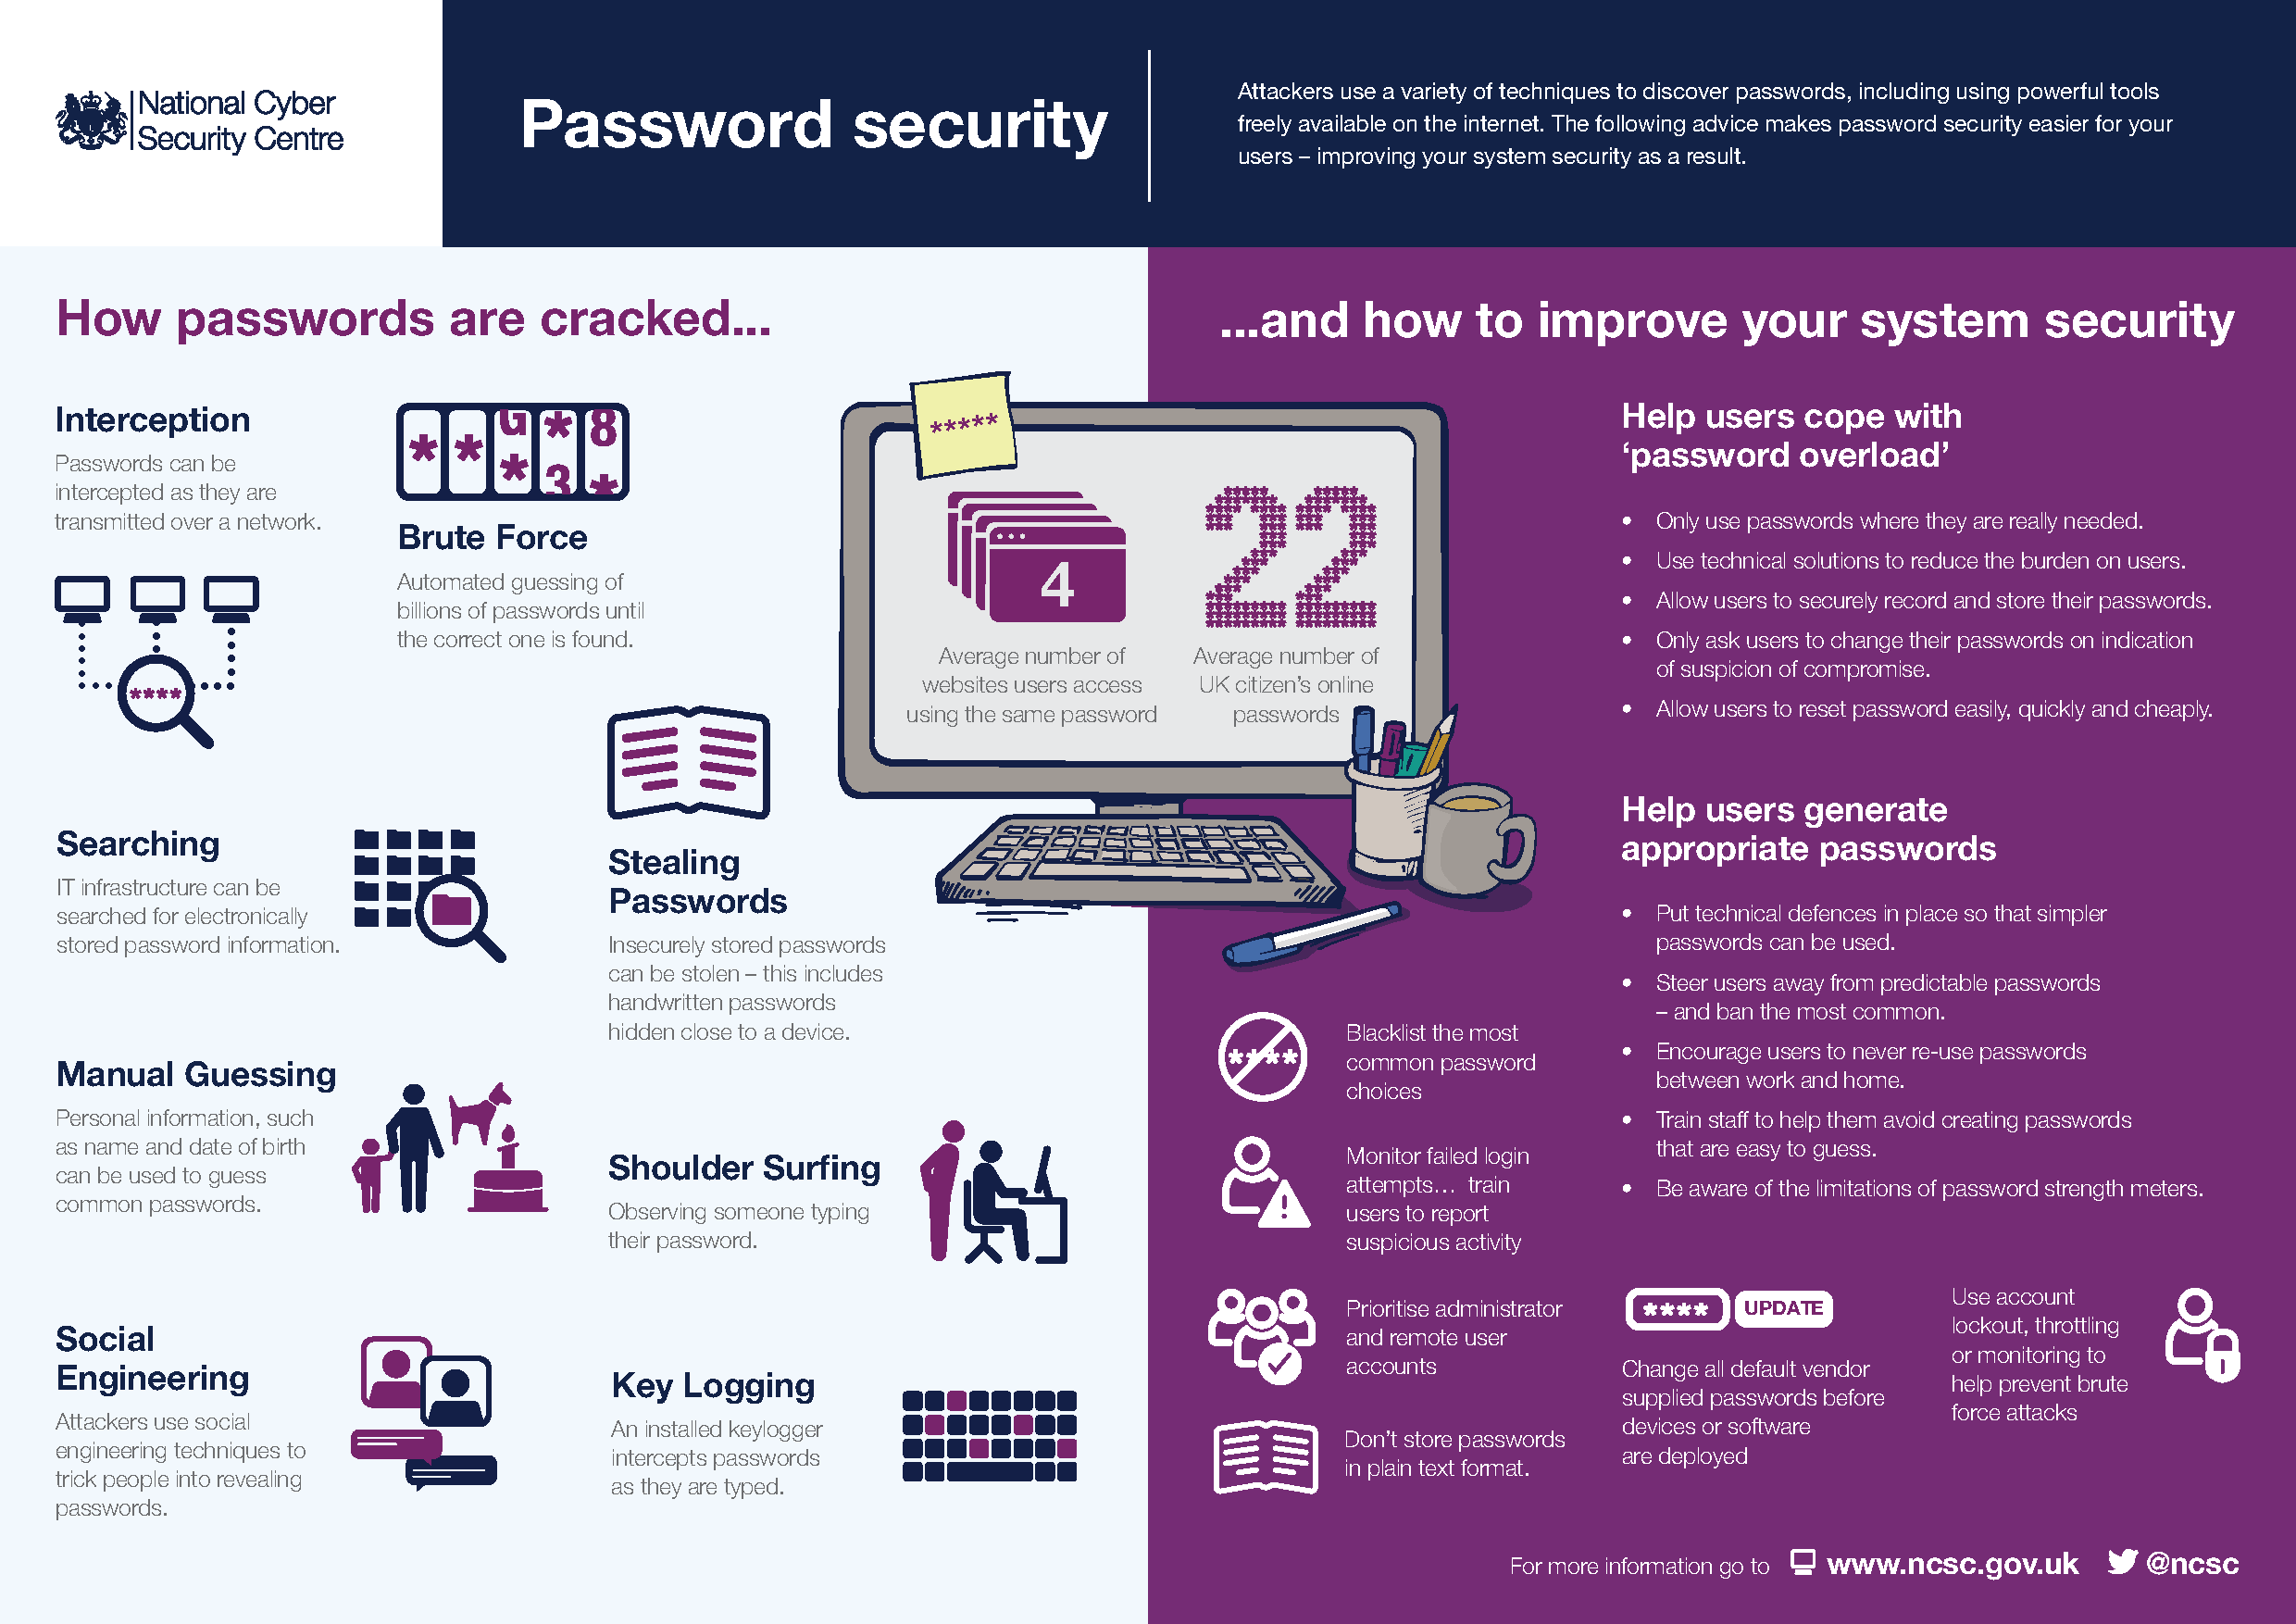
\includegraphics[width=\linewidth]{rw/NCSC-password-security-infographic}
	\caption{
		\label{fig:rw:attacks_infographic}
		Overview of attacks and high-level mitigations. Image courtesy of the National Cyber Security Centre, UK \protect\url{https://www.ncsc.gov.uk/guidance/password-collection} \protect\la{21.12.2017}
	}
\end{figure}


% A short overview of the security threats:
%%%%%%%%%%%%%%%%%%%%%%%%%%%%%%%%%%%%%%%%%
%%%%
%%%% o n l i n e    g u e s s i n g
%%%%
%%%%%%%%%%%%%%%%%%%%%%%%%%%%%%%%%%%%%%%%%
\paragraph{Online Guessing} 
%Attack description.
An adversary tries to impersonate the user by trying different combinations of user names and passwords, which are sent to the authenticating service directly. If successful, the attacker can log in without the user noticing and steal personal information, act on their behalf, and try to use the credentials on other services as well. 
% countermeasures
This attack, which is commonly known as an ``online attack'', is in many cases thwarted by throttling the number of unsuccessful login attempts per account. The service provider can lock down a user account entirely after a given number of failed login attempts. Afterwards, the user either has to manually reset their password, or they need to wait a certain time until the account is unlocked and new login attempts can be made. In the latter scenario, a strategy to hamper attacks is to implement a \textit{backoff} algorithm\footurl{https://devcentral.f5.com/articles/implementing-the-exponential-backoff-algorithm-to-thwart-dictionary-attacks}{20.12.2017} as is done in computer networks, e.g. in the Ethernet protocol \cite[p. 285]{Tanenbaum2011ComputerNetworks}. The idea behind this scheme is to (exponentially) increase the time a user (or attacker) has to wait until they can log in again after the account is locked down. Brostoff and Sasse suggest allowing ten attempts until the account is locked \cite{Brostoff2003TenStrikes}. This should give users enough trials to recover go through their list of passwords which is usually shorter than ten \cite{Florencio2007LargeScaleStudyPasswordHabits}. 
% feasibility: low, scalable but not much.
Perhaps, online guessing is only feasible for determined attackers who target specific victims, but this type of attack is not entirely uncommon \cite{Florencio2013WhereDoAllTheAttacksGo, Florencio2014PasswordPortfoliosFiniteUser, Herley2015Counterfactuals, Wang2016TargetedGuessingUnderestimated}. It is sometimes argued that such an attacker might automate up to 1 Million guesses until the attack becomes infeasible because it would simply take too long \cite{Bonneau2015ImperfectAuthentication, Florencio2014AdministratorsGuide}. However, if login attempts are not throttled, this can lead to massive attacks, like the largest attack on WordPress to date in December 2017\footurl{https://www.wordfence.com/blog/2017/12/aggressive-brute-force-wordpress-attack/}{21.12.2017}. 
% what can users do: 
Florêncio \etal argue that users are well advised to pick passwords that can at least withstand this type of attack, because it becomes too difficult to fend off offline guessing anyhow \cite{Florencio2014AdministratorsGuide, Florencio2014PasswordPortfoliosFiniteUser, Florencio2016CommACM}. 


%%%%%%%%%%%%%%%%%%%%%%%%%%%%%%%%%%%%%%%%%
%%%%
%%%% s t e a l i n g // o f f l i n e    a t t a c k s
%%%%
%%%%%%%%%%%%%%%%%%%%%%%%%%%%%%%%%%%%%%%%%
\paragraph{Stealing / Offline Guessing} Since online attacks are often impractical due to time consumption, offline attacks have prevailed in recent years\footurl{http://breachlevelindex.com/}{20.12.2017}. 
% scenario and high level description how this attack works
In this scenario an attacker breaks into the server of a service provider, usually by exploiting security holes. If this goes unnoticed, the intruder can often access the entire database containing the user account data. He or she downloads the data to their own machine, which allows them to use cracking tools like John the Ripper\footurl{http://www.openwall.com/john/}{20.12.2017}, or hashcat\footurl{https://hashcat.net/hashcat/}{20.12.2017}. These sophisticated tools use dictionaries, mangling rules and brute force to calculate password hashes which are then compared to the entry in the database. If the hashes match, the password was cracked and its plain text version is written to a file. 
% how a service provider would need to protect the data.
Optimally, the passwords in the database are salted and hashed with a slow hash function like bcrypt \cite{Provos1999bcrypt}, which drastically reduces an attacker's chances to crack the password. At the other side of the spectrum, the passwords could be stored in plain text, which would not require any cracking automation at all. Unfortunately, some of the most famous data leaks revealed that data was stored in plain text. 
% real-world examples of data breaches. first: plain text leak at RockYou
The RockYou breach in 2009 contained 32 Million user accounts for its gaming website with plain-text passwords \cite{Bonneau2012ScienceOfGuessing, Weir2010MetricsPolicies}. At the time, RockYou developed games for MySpace and Facebook and the database also contained credentials for these sites\footurl{https://techcrunch.com/2009/12/14/rockyou-hack-security-myspace-facebook-passwords/}{20.12.2017}, which made the leak even more severe. Strong passwords would not have helped at all to avoid losing personal data. Perhaps RockYou's loose policy (5 characters) helped in safeguarding other accounts where more complex policies were in place, because users were not able to reuse their RockYou password there. 
% hashed leaks
In other instances of stolen password databases, the passwords were indeed hashed, e.g. the infamous LinkedIn breaches\footurl{http://fortune.com/2016/05/18/linkedin-data-breach-email-password/}{20.12.2017} -- again with millions of rows of user data \cite{Huh2017TooBusy}. 
% User perspective: it's hard or nearly impossible. 
Users are challenged to find a password that withstands this kind of attack. The large issue is that attackers are basically only limited by the time they want to spend calculating password hashes \cite{Block2017EconomicsOfflineCracking}. On modern machines with a single GPU, thousands of hashes can be calculated per second even for slow algorithms\footurl{https://gist.github.com/epixoip/9d9b943fd580ff6bfa80e48a0e77520d}{20.12.2017}. Perhaps, this is why Florêncio \etal argue that it is futile to encourage users to pick a password that would withstand such an attack \cite{Florencio2014AdministratorsGuide, Florencio2016CommACM}. 
%TODO what happens after a breach?

%% PHISHING WEBSITE SCREENSHOT
\begin{figure}[h!]
	\centering
	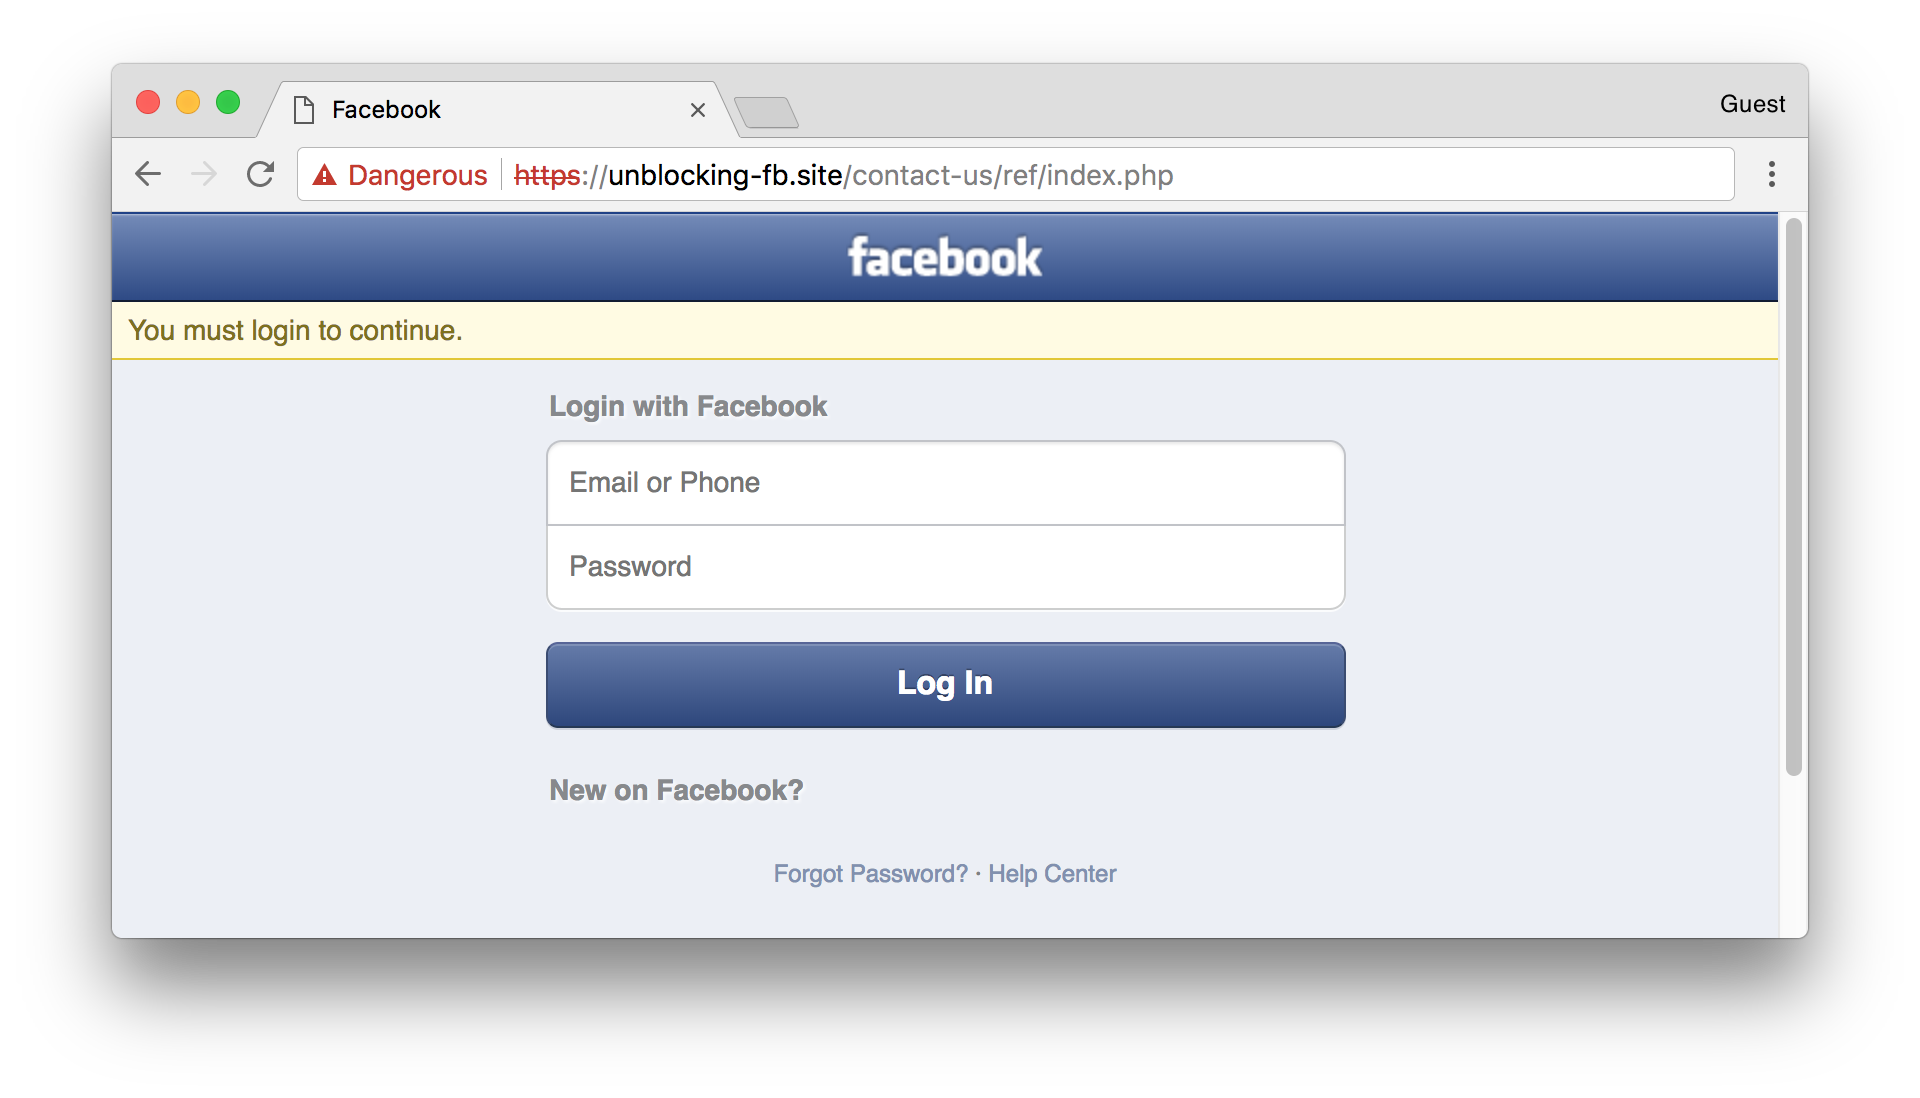
\includegraphics[width=0.7\linewidth]{rw/facebook-phishing-site}
	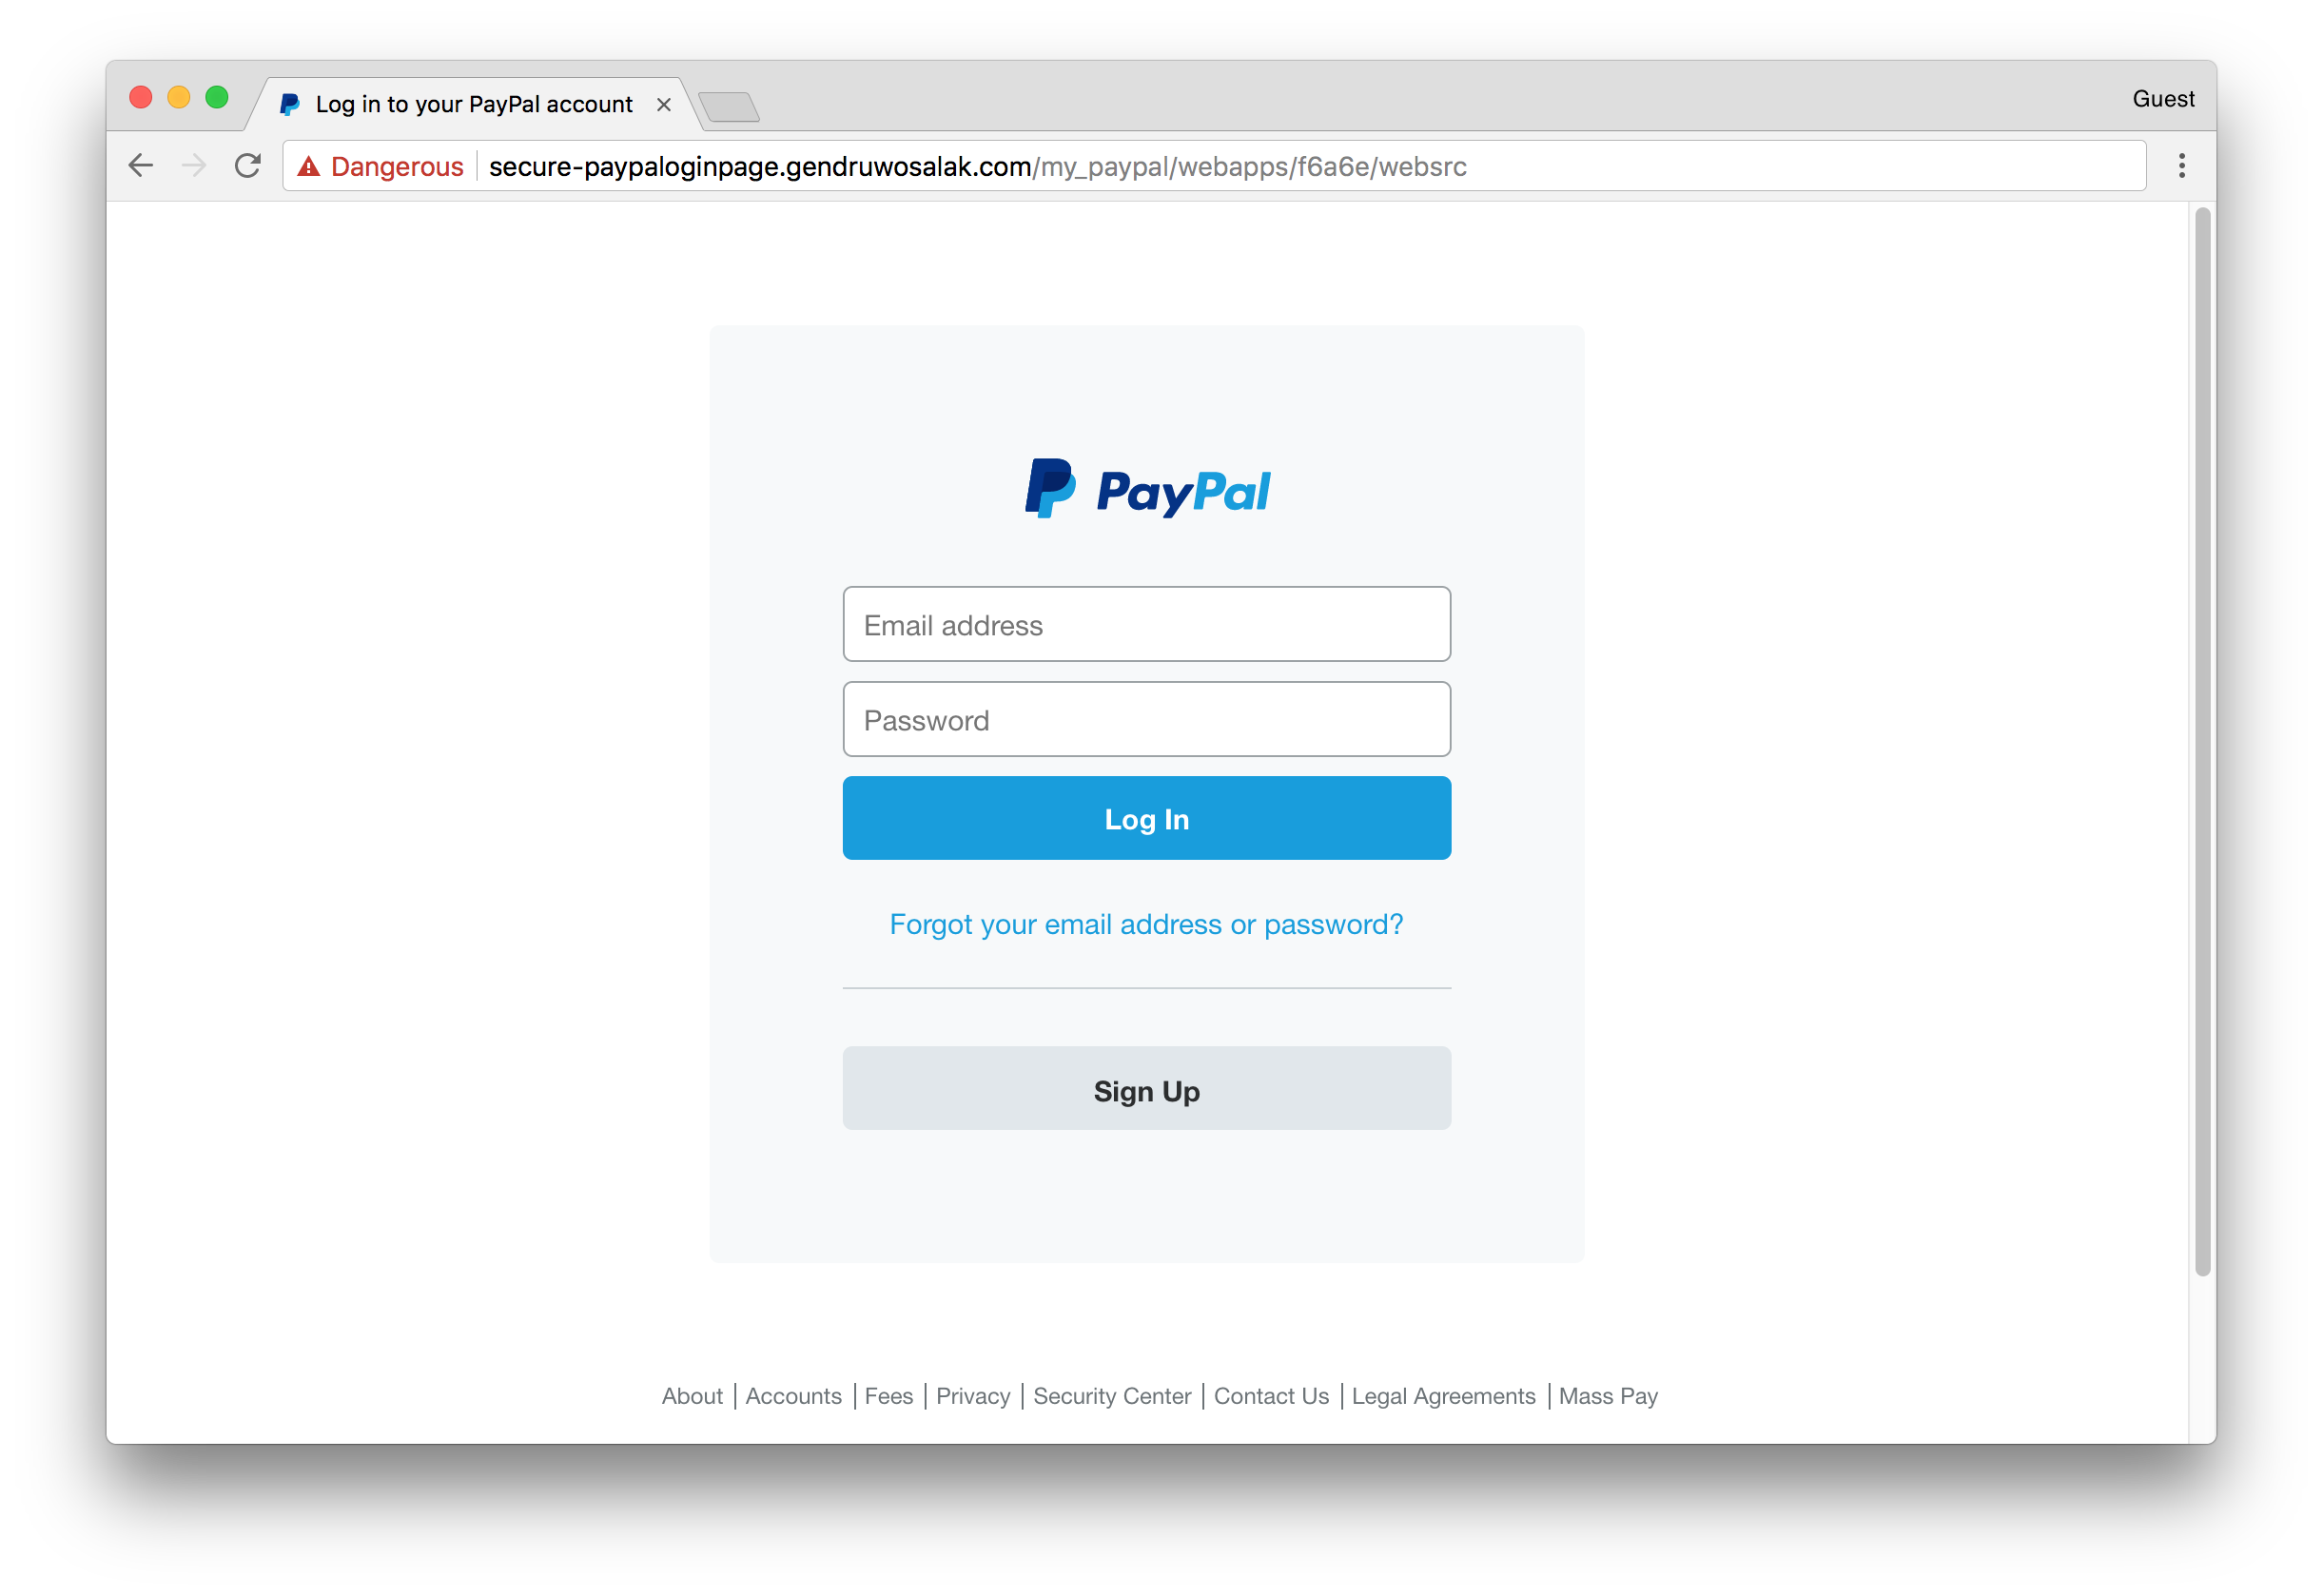
\includegraphics[width=0.7\linewidth]{rw/paypal-phishing-site}
	\caption{\label{fig:rw:phishingsite} Actual phishing websites targeting the facebook and paypal (online and accessible on 21.12.2017). The URLs contain ``fb'' (short for facebook) and keywords like ``secure'' ``paypal'' which contribute to falsely trusting the authenticity of the sites.\todo{propably split into two figures}}
\end{figure}

%%%%%%%%%%%%%%%%%%%%%%%%%%%%%%%%%%%%%%%%%
%%%%
%%%% p h i s h i n g
%%%%
%%%%%%%%%%%%%%%%%%%%%%%%%%%%%%%%%%%%%%%%%
\paragraph{Phishing / Social Engineering} 
% definition / high level description
Social engineering has become one of the biggest threats for a user's passwords with a growing number of incidents and fierce financial damage \cite{BKA2016Bundeslagebild}. Former criminal hacker Kevin D. Mitnick, who calls himself a social engineer, defines the term like this:
\begin{quotation}
	``Social Engineering uses influence and persuasion to deceive people
	by convincing them that the social engineer is someone he is not,
	or by manipulation. As a result, the social engineer is able to take
	advantage of people to obtain information with or without the use of
	technology.'' \cite[Frontmatter]{Mitnick2003ArtOfDeception}
\end{quotation}
Put simply, an attacker fools a victim into revealing certain kinds of information, including passwords. The most common social engineering attack on passwords is phishing, which typically involves two components: a fraudulent website that mimics another service and an email that lures the user onto this website \cite{Dhamija2006WhyPhishingWorks,Sheng2010WhoFallsForAPhish}. The email usually utilizes persuasive techniques like scaring  (``we noticed someone logged into your bank account and you need to reset your password'') time pressure (``you need to act \textit{now} to avoid further damage''). If the website looks just like the original (like the webpage in Figure \ref{fig:rw:phishingsite}), users might fall for it and enter their password to log in. In that case, it does not matter whether it is a strong, complex password or simply 12345 -- the attacker knows the username/password combination from that point on \cite{Tari2006ShoulderSurfingComparison}. If this tuple is used on other services, the attacker immediately gains access to them as well. 

% user perspective and mitigations
It is very challenging for users to validate the authenticity of a given webpage \cite{Dhamija2006WhyPhishingWorks, Fogg2001WhatMakesSitesCredible}. Usually, the URL is the best indicator, Dhamjia \etal among others argue that it is unrealistic to keep an eye on the URL at all times. Since the URL and padlock-icons are often ineffective, much research has been dedicated to help users in this validation and prevent phishing attacks. For example, Lin \etal found that domain highlighting in the URL bar only has a small effect on the effectiveness of phishing attacks, even after their participants were explicitly instructed to take not of the URL \cite{Lin2011DomainHighlighting}. Wu \etal showed that browser toolbars do not really help users, either \cite{Wu2006SecurityToolbars}. Dhamija \etal proposed a \textit{trusted path} between the user and the legitimate service \cite{Dhamija2005DynamicSecuritySkins}. In this system, users are supposed to verify the authenticity of a given website by comparing visual patterns in a trusted window and on the website. Together with Max-Emanuel Maurer and Alexander De Luca, I created a browser extension to visualize the usage of different types of SSL certificates across websites through the entire browser skin \cite{Maurer2011ShiningChrome}. We deployed it publicly and launched a feedback survey, which indicated that changing the browser skins is obtrusive enough to raise awareness and makes users more confident while browsing the Web. Until the recent change of platform APIs\footurl{https://blog.mozilla.org/addons/2017/11/20/extensions-in-firefox-58/}{21.12.2017} and resulting incompatibility problems, the extension named ``SSLPersonas'' had seen 47000 downloads, which is an indicator of both the necessity and the success of our solution. 

%% better solution: Browser prevents it by blocking phishing sites
However, optimally the browser would detect phishing websites and prevent that users visit them in the first place. Current versions of the major browsers try to do this and urge the user to leave the site, as is shown in Figure \ref{fig:rw:browser_warning}. This gives attackers only a short time-frame until the webpage has been classified as phishing, which takes around 4-8 hours according to a recent Webroot report \cite{Webroot2017PhishingReport}. Older sources report a bit longer lifespans between 20 hours\footurl{https://www.lightbluetouchpaper.org/2007/05/16/how-quickly-are-phishing-websites-taken-down/}{21.12.2017} and 54 hours\footurl{https://news.netcraft.com/archives/2004/08/14/life_span_of_a_phishing_site_averages_54_hours.html}{21.12.2017}. 

%%%%
%%%% Browser Warning deceptive website.
\begin{figure}
	\centering
	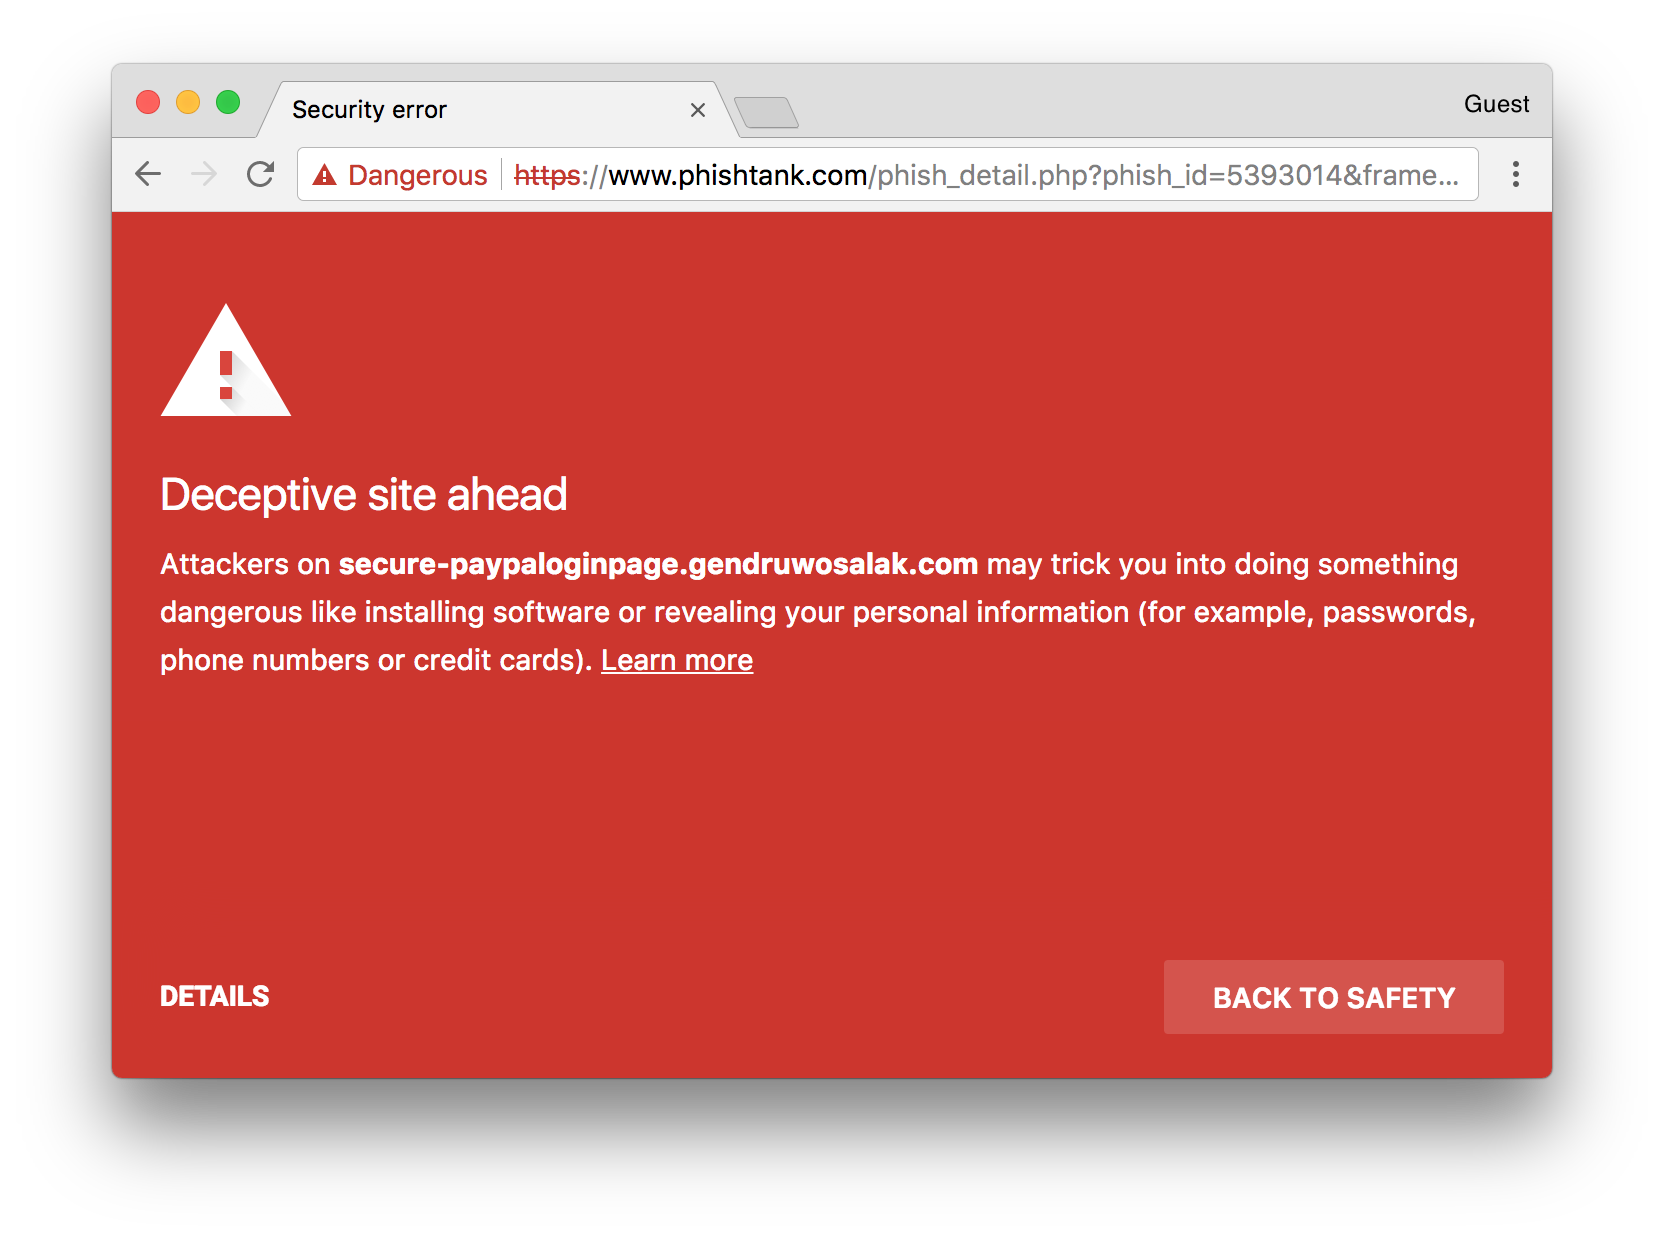
\includegraphics[width=0.8\linewidth]{rw/browser-warning-deceptive-site}
	\caption{\label{fig:rw:browser_warning}Chrome v63's warning on a phishing website. The user is urged to leave the site but still has the chance to visit it by clicking on ``Details''.}
\end{figure}

%%%%%%%%%%%%%%%%%%%%%%%%%%%%%%%%%%%%%%%%%
%%%%
%%%% m a l w a r e
%%%%
%%%%%%%%%%%%%%%%%%%%%%%%%%%%%%%%%%%%%%%%%
\paragraph{Malware and Eavesdropping} 
% attack description and types: keylogger.
Secretly stealing plain-text passwords is also possible by infiltrating the user's system with \textit{malware}, which is a term for \textit{mal}icious soft\textit{ware} \cite{Bayer2009CurrentMalware}. One of most common attacks is to install a keylogger that sends all keystrokes to the attacker. For the most part, this either happens as a ``drive-by-download'' when the user visits an infected website or by opening a malicious email attachment \cite{BKA2016Bundeslagebild}. In the former scenario, the sole line of defense lies with the service provider who needs to make sure their website is not infected.
% user perspective
Wash identified that users are aware of this kind of threat, but their mental model of malware is sub-par \cite{Wash2010FolkModels}. Hence, the countermeasures taken by the users are often insufficient. As with the phishing scenario, a strong password is incapable of preventing a malware attack. Ideally, users use an anti-virus solution, keep their software updated at all times and refrain from opening suspicious email attachments. 

% man in the middle attakcs
Moreover, user credentials can be intercepted in transit, e.g. after the user submits them through a web form. These so called man-in-the-middle attacks are tough to carry out, but strong passwords do not prevent them either. 
% solutions
One of the typical solutions to minimize the risk is encrypting the traffic with a secure protocol like SSL/TLS \cite[p. 853ff.]{Tanenbaum2011ComputerNetworks}, which is based on a public/private key infrastructure. This makes it harder for an adversary to act as the man in the middle, because they usually do not possess the necessary private key of either party. Attackers must tamper with the certificates which usually causes browsers show a warning \cite{Maurer2011ShiningChrome}. 
% user perspective 
Users, however, do not necessarily understand such warnings, because their understanding of the technical details is low \cite{Herley2009SoLongThanksExternalities, Whitten1999WhyJohnnyCantEncrypt}. Consequently, the HCI community has invested much effort to convey the essential messages in a clear and actionable way \cite{Felt2015ImprovingSSLWarnings, Felt2014ChromeSSL,  Maurer2011ShiningChrome, Sotirakopoulos2011ReplicationSSLWarnings, Sunshine2009CryingWolf}.

%Keyloggers, eavesdropped communication (e.g. via Man in the Middle Attacks)

%%%%%%%%%%%%%%%%%%%%%%%%%%%%%%%%%%%%%%%%%
%%%%
%%%% o b s e r v a t i o n 
%%%%
%%%%%%%%%%%%%%%%%%%%%%%%%%%%%%%%%%%%%%%%%
\paragraph{Observation} 
%what's the problem? how does the attack work? what are countermeasures from a technical side? what are countermeasures for the users? do strong passwords help? skill level required by the attacker?
To obtain the password of a specific user, one can also simply watch them enter it and figure out what the password was. This attack is typically referred to as ``shoulder surfing'' because the person who watches figuratively ``surfs'' on the user's ``shoulder'' to look at their screen \cite{Tari2006ShoulderSurfingComparison}. Shoulder surfing is relatively easy and does not require technical sophistication. But, although friends and family can carry out such an attack, it is safe to say that it is more problematic in public spaces where unknown bystanders are present. Typical interactions that take place in such environments can be found with PIN entry, e.g. on an ATM, or entering any kind of password on a mobile device, e.g. on a bus in close vicinity to other people. 
% new system as countermeasure: De Luca / ColorPIN
De Luca \etal dedicated some research to both scenarios. For instance, they investigated contextual factors during ATM usage and the design space for alternative ATM authentication mechanisms \cite{DeLuca2010UnderstandingATMSecurity}. They developed the ColorPIN scheme \cite{DeLuca2010ColorPIN}: Additionally to the number sequence, the user needs to memorize a \textit{color} sequence, e.g. 1 (\textbf{black}) - 2 (\textbf{red}) - 3 (\textbf{white}) - 4 (\textbf{black}). \todo{it would be nice if the text were in that color too} Entering the PIN is done through indirect input: Instead of prompting the user to enter the digits directly on the keypad, the system displays digits accompanied by three distinct letters in black, red, and white underneath. The keyboard through which the ColorPIN is entered, shows each letter three times -- once in each color. To enter the ColorPIN, the user needs to first identify the correct digit (e.g. ``1''), and then type the corresponding letter in the right color (e.g. a black ``Q''). After each entered character, the letter assignment is randomized again. All of this makes it challenging for a shoulder surfer to quickly observe and learn the user's PIN by overwhelming their short-term memory \cite{Dunphy2010CloserLookGraphical}.

% it's mostly PINs and graphical passwords rather than alphanumeric ones
Moreover, long alphanumeric passwords are a seldom research topic with regard to shoulder surfing. Shaub \etal looked into the effect of different designs of virtual keyboards on shoulder surfing susceptibility \cite{Schaub2012PasswordShoulderSurfing}. Somewhat unsurprisingly, they found that keyboards with more cumbersome access to special characters are less prone to shoulder surfing. We can see in the ColorPIN example, PINs and graphical passwords are more perceived to be under attack. Users usually enter graphical passwords more slowly \cite{Tari2006ShoulderSurfingComparison, Wiedenbeck2006ConvexHull, Renaud2009VisualSnakeOil}, which on the one hand gives an attacker more time to observe, but on the other hand burdens the short-term memory a bit more. Also, some visual authentication mechanisms require more screen real estate than a username/password form and entry is often not masked \cite{Biddle2009GraphicalFirstTwelveYears}. Still, there is not a lot of evidence that observation is a severe threat in the real world, other than for ATM PINs and any kind of credentials of people of public interest. Herley and Pieters point out that the attack is not scalable via algorithms like offline guessing \cite{Herley2015Counterfactuals}. Hence, Maguire and Renaud come to the conclusion that ``shoulder-surfing may well be a non-issue in authentication design'' \cite{Maguire2012YouOnlyLiveTwice}. 
% what about shoulder surfing on the web?
In the same On the web, observation is rarely a major concern. 



not only passwords but anything that you do on a computer can be shoulder surfed, e.g. text messages \cite{Eiband2016MyScrawl}.


typically graphical password schemes are more concerned with this attack, because the screen real estate needed to display and enter them is usually higher.  \cite{Tari2006ShoulderSurfingComparison} 
in general the attack is prevalent with authentication in public spaces, e.g. atms or on mobile devices. \cite{DeLuca2013BackOfDevice} \cite{Roth2004PINShoulderSurfing} PINs are easier to observe than pws because they are shorter and only numerical -- realistically for atms, where a two factor system is in place an attacker first needs to observe the pin and then steal the hardware token (magnetic strip cards)

On screen keyboards: De Luca \etal displayed multiple cursors on screen that acted as distractors. For users it was easy to recognize the actual mouse cursor 
\cite{DeLuca2013FakeCursors}


Shoulder surfing, passwords on post-its at the office. that's why passwords are masked in the browser (with an asterisk per character), but the benefit has recently been questioned \cite{Sasse2016DebunkingMyths}. 



%%%%%%%%%%%%%%%%%%%%%%%%%%%%%%%%%%%%%%%%%
%%%%
%%%% o t h e r    a t t a c k s
%%%%
%%%%%%%%%%%%%%%%%%%%%%%%%%%%%%%%%%%%%%%%%
\paragraph{Other attacks} 
Apart from the attacks described above, there are other approaches that should not go unmentioned. First, people in one's own social circle, e.g. friends and family, have much personal information and often physical access to devices and passwords written onto post-it notes. Although the intent is often not purely malicious, it can be easy for these people to have an informed guess of a user's credentials. Flechais \etal use the term ``spouse attack'' to describe this kind of threat \cite{Flechais2013SaudiArabiaTrust}, Dunphy \etal call it a . Ur \etal found that users underestimate its likelihood \cite{Ur2016PerceptionsPassword}. A strong, complex password that is only memorable to the legitimate user might help in that scenario. Weirich and Sasse, however, argue that such a strategy could make the user appear ``paranoid'' \cite{Weirich2001PrettyGoodPersuasion} and Flechais \etal see it as an important sign of trust \cite{Flechais2005DivideConquerTrust, Flechais2013SaudiArabiaTrust}. 
 
%%%% unintentional disclosure
Finally, some credentials are shared unintentionally on the web. Software developers who share open source code on the web are prone to this issue. Recently, the node package manager (npm) platform realized that many of its users published their passwords with the packages\footurl{http://blog.npmjs.org/post/161515829950/credentials-resets}{22.12.2017}. An adversary could simply crawl public repositories on GitHub and collect the passwords in plain text. The npmjs.org operators had to invalidate the credentials to secure the accounts. One solution that reduces the severity of credential loss is using multi-factor authentication (cf. Section \ref{sec:rw:shared_auth_tokens}).


%%%% 
%%%% TABLE: Attacks and Countermeasures
% Table generated by Excel2LaTeX from sheet 'attacks-mitigations'
\begin{table}[htbp]
  \centering
  \caption{\label{table:rw:attacks_countermeasures}Threats on passwords and potential countermeasures for users and service providers (SP). Other stakeholders are left out of this analysis.}
    \begin{tabular}{rll}
    \multicolumn{1}{l}{\textbf{Threat}} & \textbf{Countermeasures} & \textbf{Responsible} \\
    \hline
    \multicolumn{1}{l}{\textbf{Online Attack}} & Throttling & SP \\
          & Anomaly detection & SP \\
          & Set-up Multi-factor authentication & SP \\
          & Moderately complex password & User \\
          & Enable Multi-factor authentication & User \\
    \multicolumn{1}{l}{\textbf{Offline attack}} 
        	& Slow hash algorithm & SP \\
			& Secure database design & SP \\
			& Security audits, fix vulnerabilities & SP \\
		    & Complex, strong password & User \\

    \multicolumn{1}{l}{\textbf{Phishing}} & Education and Warnings & SP \\
    & Unique passwords & User \\
          & Check security indicators & User \\
          & Utilize spam filter & User \\
          & Vigilance regarding emails & User \\
    \multicolumn{1}{l}{\textbf{Malware}} & Anti-Virus software & User \\
          & Caution on the web & User \\
    \multicolumn{1}{l}{\textbf{Observation}} & Password masking & SP \\
    	& Awareness of surroundings & User \\
    \end{tabular}%
\end{table}%
\todo{make this more convincing}
%%%%
%%%%

%TODO Florêncio \etal proposed a classification for attacks \cite{Florencio2014PasswordPortfoliosFiniteUser}. Class 1-3

%TODO what is an attack ``vector''? attack steps from start to success. \ar
%Sometimes combinations of attacks (vector)

The main objective of this thesis is combating online and offline attacks, i.e. for algorithmic attacks, where password coping strategies really make a difference. A panacea for all kinds of threats, each of which has warranted multiple PhD theses, is probably impossible to find. 



%%%%%%%%%%%%%%%%%%%%%%%%%%%%%%%%%%%%%%%%%
%%%%
%%%% w h a t    i s    p a s s w o r d    s t r e n g t h
%%%%
%%%%%%%%%%%%%%%%%%%%%%%%%%%%%%%%%%%%%%%%%
\section{What is Password Strength? - Metrics and Statistics}\label{sec:rw:pw_strength_metrics}
Bishop and Klein said in 1995: ``A good password is one that is easily remembered, yet difficult to guess.'' \cite[p. 231]{Bishop1995ProactivePasswordChecking}. The second part of this statement describes password \textit{strength} on a high level. But there are problems if we try to objectively measure the ``difficulty to guess'' a password: is it difficult for an attacker with nearly unlimited resources, or only for an attacker that can only attempt once a day due to lock-out mechanisms? The question is highly context dependent and there is unfortunately no single true answer. 

How to attack passwords
- here the most important paper is:
Cracking techniques must be used in parallel to get the complete picture of password guessability \cite{Ur2015MeasuringRealWorldAccuracies} -- mention tools like HashCat/oclHashcat, John The Ripper 

give some real world examples how passwords are attacked online and how they have been attacked offline. 


Lately the community reached widespread consensus that the realistic strength of password can be defined as \textit{the number of attempts that an attacker would need in order to guess it} \cite{Dellamico2015MonteCarlo}

 

Don't forget: Password strength is dynamic! New leaks can render strong passwords very weak. Yang \etal state: ``If a strategy is widely used, then attackers may develop strategy-specific methods which can efficiently guess the passwords.'' for example: if passphrases do become commonplace, attackers will optimize their attack strategy. in the end, the number of leaked passwords will continue to grow so it is tedious to ``outrun'' hackers by resetting passwords etc.

Bonneau looked at leaked passwords and tried to attack them in different ways to find patterns in user behavior that could be leveraged in real-world attacks \cite{Bonneau2012ScienceOfGuessing}. Fundamentally, the attacks were based on different dictionaries. He found that the success rates of attacks strongly depend on the dictionary that is used for it. Under the assumption that entropy is a viable strength proxy, he concluded that 10 bits of entropy are probably enough to defend against online attacks, respectively 20 bits for offline attacks. 

\cite{Peisert2013PriciplesAuthentication,Bonneau2012ScienceOfGuessing,Scott1995GDMS,Dellamico2015MonteCarlo,Ur2015MeasuringRealWorldAccuracies,Egelman2015SeBIS,Conklin2004PWAuthenticationSystemPerspective,Schmidt2013Pitfalls,Kelley2012GuessAgain,Mazurek2013Measuring,Weir2010MetricsPolicies}

	\subsection{Entropy vs. Guesswork}
	
	Other definitions: ``The strength of a password should represent the amount of effort an adversary must employ to break the password'' \cite{Carnavalet2014AnalyzingPWStrengthMeters}.
	
	William Burr regrets NIST policy (see footnote \ref{foot:burr_regrets})	
	
	
	
	Entropy (Shannon) -- degree of randomness. often too focused on characters and doesn't address human password selection, which is far more predictable 
	(effective vs. theoretical password space)
	
	@@TODO tell the story of all the attacks -- Kelley, Weir, Bonneau, Melicher, Johnson, Ur etc. Password Guessability Service etc. 
	
	Leaked password dictionaries: Most commonly: RockYou (gamer site), MySpace, LinkedIn, Gawker, Yahoo!
	Mark Burnett  \cite{Burnett2005PerfectPasswords} 
	
	Tell the history of how guesswork was modeled. Starts out with \cite{Weir2010MetricsPolicies}, then \cite{Kelley20012GuessAgain} and \cite{Bonneau2012ScienceOfGuessing}. 
	
	Weir et al established a guessing method where the most probable passwords are tried first (PCFG) and measure how many passwords can be cracked until a cut-off threshold, and this resulting metric is more valid than entropy \cite{Weir2010MetricsPolicies}
	
	NIST entropy was THE measure for password strength until the Weir paper and shortly afterwards. \cite{Komanduri2011OfPasswordsAndPeople} is probably the last CMU paper that uses entropy as strength metric (and is proud of it).
	
	Entropy is relative to / dependent on a given set of passwords. 
	
	Passfault can crack passwords and is open source \cite{Paiva2017Passfault}
	
	Neural networks perform really well to crack passwords if you configure them correctly and you can even do this in the browser, but it's not super trivial \cite{Melicher2016NeuralNetworks}
	
	\subsection{Beta-guess-rate}
	$\lambda_{\beta}$
	quasi: how likely is it to find the top $\beta$ passwords in a given dataset?
	see bonneau, and also used in \cite{Yang2016MnemonicSentenceBased}
	brostoff and sasse  proposed 10 as a threshold for rate-limiting (before account is locked and password invalidated until reset) \cite{Brostoff2003TenStrikes}
	
	
	
	
	\subsection{Strength Proxies: The zxcvbn Approach}
Daniel Wheeler presented an approach towards password strength estimation by looking at a conservative expected guess attempt number \cite{Wheeler2016zxcvbn}. The idea is to utilize pattern matching against dictionaries and leaked password corpora and then calculate the minimum rank over a series of frequency ranked lists. In other words, the approach is heuristic instead of probabilistic, because the ranking is based on searching through the patterns and ranking them not only based on their likelihoods, but other factors like keyboard sequences. The implementation of the algorithm is called zxcvbn\footnote{The name zxcvbn originates from the bottom row on a QWERTY keyboard. Many users mistakenly consider this approach secure because the resulting password looks fairly random.}. Wheeler showed that in an online attack scenario \cite{Florencio2014AdministratorsGuide} the algorithm estimates the number of guesses accurately within an order of magnitude of 2 -- consistently better than NIST guidelines to date and KeePass strength estimators. That is, utilizing 100,000 tokens stored within a 1.5 Megabyte file zxcvbn conservatively estimates the number of guesses required to crack a password. Beyond the online-attack threshold, the results are mixed, but we can observe that adding more tokens to the dictionary improves accuracy even more. The great benefit of using this method is its speed and size that make it a lightweight tool that is prepared for widespread adoption, to relieve users from ``LUDS'' policies (lowercase, uppercase, digits, symbols). We can conclude that zxcvbn is a reasonable tool when we collect meta statistics about passwords, e.g. in studies where it is ethically questionable to collect plain text passwords \cite{Seitz2016SuggestionsDecoy}. Wheeler also points out that at this point there is no study comparing the effects the different estimators have on user behavior. 

papers that used or mentioned zxcvbn:
\cite{Komanduri2014Telepathwords}
\cite{Wang2016fuzzyPWM}
\cite{Ur2017DataDrivenPWMeter}
\cite{Yang2016MnemonicSentenceBased}
\cite{Gross2016CognitiveDepletion}

Weaknesses \cite{DeCarnedeCarnavalet2015PasswordMeters}: only english dictionary words, fixed dictionary with the constraints of being transfered to the client, so some passphrases are considered strong while they are not really super great, e.g. ``dolce\&gabana''
not true anymore but in the paper: reversed passwords are not recognized (Wheeler updated this). 


\section{What is a ``Bad'' Password?}
This question is flawed, and thus cannot be answered without context. The word ``bad'' is judgmental and depends on whom is asked. A security expert might call a password ``bad'' if it only contains lowercase letters, but a regular mainstream user might call it ``bad'' because they cannot type it quickly or can't remember it well. 

Bishop and Klein said in 1995: ``A good password is one that is easily remembered, yet difficult to guess.'' \cite[p. 231]{Bishop1995ProactivePasswordChecking}

Let's look at 

types of attacks: phishing, online (rainbow), offline, targeted online. \cite{ZhangKennedy2016RevisitingPasswordRules}. 

When does password strength really help? 

This paragraph from Herley and Van Oorschot says it all \cite{Herley2012PersistenceOfPasswords}:
``Fifth, when are off-line attacks a threat? While dependent on implementation, access to salted hashed pass- words requires attacker effort; long gone are the days when password hash files were by default world read- able. A disgruntled ex-sysadmin who steals hashed pass- words is the often-conjectured foe in this attack; yet, if un-trusted individuals have had unfettered unaudited access to the authentication server, a site’s problems go well beyond password strength. Sixth, are there ways to protect against off-line attacks besides password strength? Mandating password changes once hashes leak might be better than strong policies at all times. Only if a leak goes unnoticed (and a password change isn’t forced) does strength potentially help. Of course, reliably detecting leaks or break-ins it- self remains difficult. Finally, how much strength is required to protect against off-line attacks? The bar is clearly much higher than for online attacks (assuming lockout or rate-limiting policies in place), but at what strength are attacks effectively addressed? More strength is always better for security,'' 

discuss online and offline attacks
\cite{Wang2016fuzzyPWM} has an overview/comparison
\cite{Florencio2014AdministratorsGuide} shows models
\cite{Florencio2014PasswordPortfoliosFiniteUser} has math

A problem about only taking ``online'' attacks into account is that they do allow denial of service attacks, for example if there's lockout policy in place that invalidates passwords after 10 failed login attempts, an attacker would only need to take a list of email addresses (readily available on the internet) and run 10 or more guesses per user and lock all of them out at once. 



We shouldn't call it good or bad. A less judgmental terminology is ``strong'' and ``weak'' because this doesn't include opinions. 

A ``strong'' password is one that cannot be guessed easily by a human or a machine, regardless of the level of information they have about the owner of the password. 


The idea behind a PCFG based policy is to reject passwords that are too ``probable''. 

Characteristics of weak passwords \cite{Burnett2005PerfectPasswords}
\begin{enumerate}
	\item Are used by many users
	\item Can be found through an internet search
	\item Are short (6 characters or less)
	\item Have leaked
	\item Are written down where anyone can access them
\end{enumerate}

But there are other, non-technical qualities of passwords that are usually not covered by the weak-strong spectrum. 

When is a password \textbf{``Appropriate''}? This largely depends on the usage context. \cite{Gaw2005ReuseRecycle, Haque2014Hierarchy}
Florencio \etal argue that it is absolutely fine to choose a weak password for ``don't-care'' accounts \cite{Florencio2014}.

Requirements from a user perspective: memorable and easy/fast to type on all devices.

this creates tensions that are discussed in detail in Chapter \ref{chap:rw:user_perspective}.


\section{Authentication beyond Passwords}\label{sec:rw:authentication_without_pws}
The benefits and drawbacks of using passwords have been studied extensively. Some drawbacks already become apparent when we recall Ali Baba's story: Ali Baba overhears the thieves saying the magic words and can immediately authenticate with them (a big security issue). He also told the ``password'' to his brother, but he fails to recall it (the biggest usability issue).

Table \ref{table:rw:benefits_drawbacks_pws} shows a high-level summary of the benefits and drawbacks that come along with password-based authentication. We can observe that the drawbacks constitute important constraints and it is natural to try to remove such limitations by considering alternatives. This section briefly covers the most notable approaches to authenticate users without alphanumerical passwords.

\begin{table}
	\begin{tabular}{|l|l|l|}
		Benefits | Drawbacks 
	\end{tabular}
	\caption{\label{table:rw:benefits_drawbacks_pws}Benefits and Drawbacks of passwords for different stakeholders}
\end{table}
%benefits: easy to implement, users know how they work, concept is easy to learn, can be shared, can be replaced when they are compromised, can be revoked by the sys admin, quick to enter, work without a user name (WiFi) so it's easy to scale. 
%drawbacks: users have to cope with many passwords, so they use risky strategies \ref{sec:rw:how-users-cope}, it's difficult to manually create a password that is both usable and secure (good enough to protect against offline attacks)




% das passt nicht unbedingt hier rein, ist aber sehr wichtig. 
Bonneau et al. argue \cite{Bonneau2015ImperfectAuthentication} that passwords are an imperfect technology that is difficult to replace. One, industry has found ways to work around the many drawbacks and can compensate breaches to a large part. Second, alternatives to passwords are often privacy invasive. For example, identity providers like Google or Facebook often collect large amounts of personal data on the users. Third, Bonneau et al. point out that empirical evidence from practice often contradicts results produced by academic research. They advocate that researchers rethink their model of users, who often behave too predictably and whose behaviors one should not try to change. Instead, academia could tackle new approaches that would be dangerous to the success of businesses and thus are seldom tried out. 

% noch mehr Zusammenfassung für später:
The authors point out how user models assumed by researchers often do not apply in reality, for instance, their behavior is anything but random: Users pick from a limited set of passwords that is far smaller than random passwords. Just as \cite{Florencio2014PasswordPortfoliosFiniteUser}, the paper strongly discourages focusing on offline attack scenarios and suggests that users should at most try and protect themselves against online attack scenarios. Consequently, the lessons from the past about attempts to improve password strength through changing user behavior are questionable in the authors' eyes. Even more so, because other attacks (phishing, malware, eavesdropping, stealing from servers or identity tokens) are not fended off at all by stronger passwords. Online attacks can drastically be mitigate by rate-limiting and contextual information (e.g. geolocation). Yet, the authors see that not all sites employ these methods, ``probably to avoid denial of service''. Users also often receive too much advice from security experts that is often contradictory and in extreme cases boiled down to ``Pick something you cannot remember and do not write it down''. 

Bonneau et al. answer the question whether we still need passwords with a differentiated ``yes'': \textit{Passwords appear to be a Pareto equilibrium\footnote{\todo{add definition of this here. It's about game theory.}}}. Also the learning curves for password authentication at a new service is virtually non-existent. However, as many researchers in the community, the authors see the feasibility of multi-factor authentication in progressive or continual ways as the most promising future. The challenges for privacy and usability we find in these approaches are mostly ill-defined or not validated. The user experience of such systems may improve while the drawbacks come at a high price that the users may not understand at all. 

	\subsection{Graphical Passwords \& Visual Authentication Methods}
Graphical passwords can work for children and adults \cite{Imran2015PWsAdultsChildren}

, Ema's work, \cite{Renaud2009VisualSnakeOil} 

	\subsection{Biometrics}
	
	\cite{Jakobsson2014HowToWearYourPW,DeLuca2012TouchMeOnce,Peisert2013PriciplesAuthentication,Rybnicek2014RoadmapContinuousAuth}
	

	fingerprint omnipresent 
	retinal scan
	face recognition (iPhone X)
	
	
	Anecdote to show that it is a bad idea\footnote{\url{https://www.theguardian.com/world/2017/nov/08/qatar-airways-plane-forced-to-land-after-wife-discovers-husbands-affair-midflight}, \access{08.11.2017}}
	
	\subsection{Multimodal and Implicit Authentication}
	
	actually the technical report gives some insights about this \cite{Stockinger2011ImplicitAuthentication}, so that will inspire a bit.
	also look into the USEC folder in the office, the papers and annotations are in there.
	
		it's interesting that the most cited CHI paper of the last 5 years is about implicit authentication \cite{DeLuca2012TouchMeOnce}
		
		\cite{Roalter2013SmartphoneProxy}
	
	Machine learning. Accuracy / Recall / Error rate / True Positve / False Positives etc. -- based on \textbf{probability} and not on \textbf{certainty}. To account for the lack of certainty, in all current state-of-the-art mechanisms passwords serve as fallback authentication. So, while it reduces the number of password entries and so speeds up interactions in many cases, these schemes cannot fully replace passwords. What is worse is that the rare interaction often tempts users to choose a very memorable secret, which in most cases is weaker than a password that is entered on a regular basis. So an attacker that is successfully denied access to a system protected by multimodal authentication will always have the opportunity to authenticate with a password -- the system needs to assume a false negative and offer the fallback authentication scheme. In this scenario, while the primary authentication is more usable and very secure, the entire system's security is lowered by its fallback scheme. This fact is often played down and neglected in the marketing of new multimodal authentication. 
	
	Take away: implicit authentication cannot replace explicit authentication, but it can make an existing scheme more secure. Fallback schemes tend to lower system security. 
	

in a study setting, giving users power over their authentication scheme worked well, but it might not in real-world settings \cite{Forget2015CYOA}
	
	\subsection{Shared Authentication and Hardware Tokens}\label{sec:rw:shared_auth_tokens}
Single Sign-On (SSO). 
Identity Providers, 
SecureID or ``Gnubby'' (see Google)
Two-Factor Authentication / 2-step --> hints to 2-step in ``Some UNIX systems have instituted what is called an "external security code" that must be typed when dialing into the system, but before logging in. If this code is changed periodically, then someone with an old password will likely be prevented from using it.'' \cite{Morris1979PasswordSecurity}


If authentication mechanisms were a tournament, users would prefer OAuth and QR-Codes to authenticate, but in the real world, this isn't the case \cite{Ruoti2015AuthenticationMelee}

Reference Models:
\cite{Egelman2013ProfilePassword,Sun2010BillionKeys}

\begin{itemize}
\item \textbf{OAuth} Twitter, Google
\item \textbf{OpenID} Google, PayPal
\item \textbf{Facebook Connect} 
\end{itemize}
Problems: 
Successful identity providers such as Facebook take a central role as the ``sole identity provider, which does little for privacy'' \cite{Bonneau2015ImperfectAuthentication}.


\textbf{Privacy} The biggest players for shared authentication are Facebook, Google, and Twitter. However, it is exactly these three companies for which users raise the most privacy concerns. On the one hand, users trust the companies because they know how much data they store and manage, and only few breaches are known. On the other hand, users are doubtful that their credentials will be in safe hands and not shared with third parties (users lack the understanding of how shared authentication works internally and cannot separate privacy and security). 

\textbf{Single Point of Failure} Embracing the opportunities of shared authentication, users integrate it into their password management / coping strategies \ref{sec:rw:how-users-cope}. 

	
\subsubsection{One Time Passwords}

OTP also have the possibility to replace a password that you have to memorize, but there are disadvantages as well. 
illustrate the workflow from Slack.

Authentication Melee paper has some intel on one-time passwords: \cite{Ruoti2015AuthenticationMelee}


\section{Passwords are Here to Stay}
no solution fully replaces them

most approaches that are seen as more usable are often based on probability rather than certainty (TPR / FPR / EER). fallback to passwords probable even for other authentication schemes. everything else is often less usable than passwords. 

maybe discuss this at the end of the thesis: passwords are cool, and we can continue to use them because they are so easy to replace in case of a breach. 

An approach that is currently not undertaken in internal security audits is the following: there are password leaks once a month (see data breach reports). the security team could take the passwords (if they are hashed - crack them first) and invalidate all matching passwords in their own password database. Of course, they need to inform their users. I could sketch a flowchart what this should look like. This would allow reusing passwords more securely without shifting much responsibility to the users. 

``We argue that it is time to admit that passwords will be with us for some time, and moreover, that in many instances they are the best-fit among currently known solutions.'' \cite{Herley2012PersistenceOfPasswords} 

The Herley and Van Oorschot paper really has lots of good quotes and thoughts for this
We need a more systematic research approach about passwords to make users' lives easier and we shouldn't try to find a single scheme that replaces them (impossible) but a more triangulated approach \cite{Herley2012PersistenceOfPasswords}


\cite{Kirlappos2012SecurityEducation,Loutfi2015PasswordsOtherSideOfTheFence,DeAngeli2005PictureThousandWords,Florencio2013WhereDoAllTheAttacksGo,Herley2008ProfitlessEndeavor,Sasse2015,Dittrich2009,Herley2009SoLongThanksExternalities,Vantaggiato2015WeStillNeedPasswords,Florencio2010WhereDoPoliciesComeFrom,Schrittwieser2013,Bonneau2015ImperfectAuthentication,Cyber2014,Florencio2007DoStrongWebPasswords,Sasse2005UsableSecurityPosition,Aebischer2017PicoInTheWild,Forget2007HelpingUsers,Herley2009IfWereSoSmart,Acar2016NotYourDeveloper,Sasse2016,Renaud2009VisualSnakeOil}



%\part{PERSUASION IN USABLE SECURITY}
%!TEX root = ../../diss.tex

\chapter[Decision Making in Usable Security]{Decision Making in Usable Security}\label{chap:rw:persuasion}

Short history of behavioral economics and decision making studies

portray irrational decisions and discuss why or not password selection is rational / irrational

theory of planned behavior, intrinsic motivation, 


\section*{Related Work Overview *}
\begin{itemize}
\item Forget Papers: \cite{Forget2007PersuasionEducationSecurity} \cite{Forget2007HelpingUsers} \cite{Forget2008ImprovingPasswordsThroughPersuasion} \cite{Forget2008MemorabilityPersuasivePasswords} \cite{Forget2008PersuasionStrongerPasswords}

\item Chiasson: \cite{Chiasson2008PCCP}
\end{itemize}


\cite{Furnell2017GuidanceCompliance,Kaptein2015PersonalizingPersuasiveTechnologies,Gulenko2014PasswordsEmotion,Azevedo2012AuthenticationGame,Kroeze2012GamifyingAuthentication,Schneider2016UnderstandingPersuasiveDesign,Cialdini2003CraftingNormativeMessages,Scott1995GDMS,Kim2015MobilePersuasionTrust,Bellur2014HeuristicsUsed,Baharin2015RhythmicPersuasionModel,Adams2015MindlessComputing,Han1994PersuasionCulture,Balebako2011,Acquisti2009,Forget2007PersuasionEducationSecurity,Forget2008ImprovingPasswordsThroughPersuasion,Xu2007,Zakaria2013DesigningEffectiveSecurityMessages,Egelman2010PleaseContinueToHold,Yevseyeva2014,DiGioia2005SocialNavigationUsableSecurity,Chiasson2008PCCP,Wiafe2012,Weirich2005PersuasivePasswordSecurity,Forget2008MemorabilityPersuasivePasswords,Jeske2013,Wang2014,Weirich2001PrettyGoodPersuasion,Adjerid,Shiv2005,Wiafe2012a,Almuhimedi2015a,Radke2013,Arachchilage2013GameDesingPhishing,Ashenden2013SecurityLikeSoap,Bahr2013,Korff2014TooMuchChoice,Muscanell2014,Woodruff2014PrivacyFundamentalist,Korff2014,Goldstein2008,Forget2008PersuasionStrongerPasswords,Wang2013,Hamari2014,Jameson2011PreferentialChoice,Instructor2013,Mamduhi2012,Lockton2012CognitiveBiases,Choe,Fogg2002Persuasive,Fogg2009,Lockton2010,Hekler2013,Lockton2009,Lee2011MiningBehavioralEconomics}


Das: Social sensitivity security advice: \cite{Das2014EffectSocialInfluenceSecuritySensitivity}

\section{Cognitive Illusion and Biases}
Looking at the problem from behavioral economic point of view

another term: ``cognitive distortions''

We should keep biases in mind when designing communication about security (decisions) \cite{Garg2013HeuristicsAndBiases}

Sunk costs: \cite{Herley2012PersistenceOfPasswords} say that too many actors have invested into passwords and now adopting a new scheme is hampered by the sunk costs fallacy.


Acquisiti \etal \cite{Acquisti2017NudgesPrivacySecurity} have a journal paper that has everything in it we need...
	\subsection{Definition}
	\subsection{Scenarios}
	% availability, overconfidence, decoy, anchors, hinsight, sunk costs
	
	
	

Schneier has a really good section on the reasoning of psychological effects and biases in \cite{Schneier2008PsychologySecurity} 
	
	
\section{Persuasion and Nudging}

persuasion is amongst the top-5 most-cited topics of the past 5 years at CHI
(alternative) nobel price awarded to Daniel Kahnemann and Richard Thaler - both behavioral economists

\textbf{why persuasion for passwords?} because people are seldom motivated to invest effort voluntarily. persuasion makes alternatives more salient and attractive, but does not try manipulate people. manipulation: person should not realize their being manipulated. persuasion: the target behavior should be clear and the intention of the designer, too. 

\cite{Zakaria2013DesigningEffectiveSecurityMessages} Zakaria and Katuk make the case for persuasively framing messages


nudging people towards locking their screen \cite{Bruggen2013ModifiyngUnlockingBehavior}

	\subsection{Persuasive Authentication Framework}
	\subsection{Privacy Nudges}
	nudging privacy decisions is more prominent in the literature than nudging password decisions. 
	
	
	%%%%% CENTRAL REFERENCE::
	most prominently: Acquisiti \etal \cite{Acquisti2017NudgesPrivacySecurity} \cite{Acquisti2005PrivacyRationality}
	%%%%%

\section{Personality Traits}
	\subsection{Inventories}
	Big Five à la Costa and McCrea \cite{Costa1992NEO}
	SeBIS (Egelman)
	\subsection{Personality Heuristics}	
	\subsection{Privacy Decisions}
	\subsection{Password Personalities}
	
	
	Personality seems to be correlated with certain behavior online, primarily willingness to share and phishing susceptibility \cite{Halevi2013PilotStudyPersonality}

\section{The Persuasive Authentication Framework}


\subsection{Personalization and Individualization}
Already the PAF introduced the personality dimension for effective persuasion. Recently, Egelman and Peer advocated to use psychometric cues to contextualize privacy or security messaging \cite{Egelman2015AverageUser}. In two studies they looked at the predicting power of different psychometric scales, among which we find the five-factor model (``Big Five''), the General Decision Making Style (GDMS) or the Domain-Specific Risk-Taking scale (DoSpeRT) @@TODO dreimal Quelle. They conducted two online experiments using Mechanical Turk. In the first round they used the Ten-Item-Personality Index and correlated the scores with several privacy metrics (e.g. the Privacy Concerns Scale or the Internet Users Information Privacy Concerns scale). They realized that the Big Five model was a rather weak predictor for the different scales, which lead them up to their second experiment, where they focused on decision-making metrics. Here, they observed stronger correlations, between e.g. the rational trait of the GDMS and both PCS and IUIPC. Following these observations, Egelman and Peer interpret them as evidence that privacy attitudes originate from rational decision-making, and also from people's intuitions, which sounds paradoxical at first, but it were different respondents who produced this result. They conclude that the decision-making metrics were about three times as powerful regarding their predictive power than the big five model regarding privacy attitudes and behavior. Finally, they propose the Security Behavior Intentions Scale (SeBIS). This scale intends to isolate confounding factors when correlating personalty traits with security behavior. Also, the authors offer a number of hypotheses and unanswered research questions that highlight how little exploiting personality traits in security nudges has been investigated. 




%%!TEX root = ../../diss.tex

\chapter[Password Selection]{Password Selection}\label{chap:password_selection}






\chapter[Passwords -- A User Perspective]{Passwords -- \\
	A User Perspective}\label{chap:rw:user_perspective}
%lingo: arduous

``but his thoughts were so full of the great riches he should possess, that he could not think of the word to make it open, but instead of `Sesame,' said, `Open, Barley!' and was much amazed to find that the door remained fast shut. He named several sorts of grain, but still the door would not open, and the more he endeavoured to remember the word `Simsim,' the more his memory was confounded, and he had as much forgotten it as if he had never heard it mentioned.'' (Kasim's predicament in \textit{Ali Baba and the Forty Thieves}) \todo{this could be the opening of the chapter / fancychapter}

Morris and Thompson were already concerned with user behavior regarding passwords in 1979 \cite{Morris1979PasswordSecurity}. They identified that users choose predictable passwords and that this can be leveraged for attacks. So, they suggested enforcing a certain minimum password length (six characters). At the time, the users were mostly professionals that received training to operate computers and could thus also have been trained to pick less predictable passwords \cite{Maguire2012YouOnlyLiveTwice}. But as computers were introduced to a larger audience, more people were exposed to password authentication. Naturally, this also induced a growing number of attacks, and it is increasingly difficult for users to defend themselves against them (see. Section \ref{sec:rw:attack_vectors}). Nowadays, password policies are in place that require not only a minimum of eight characters, but also mandate mixed-case letters, digits and special symbols to start with. The HCI community noticed the users' struggle in the 1990s and that we can -- and should -- design authentication systems with usability in mind. Perhaps, one of the breaking points where a new school of thought turned up in the literature was a paper by Adams and Sasse in 1999 \cite{Adams1999UsersEnemy}. The central and novel theme in there was a shift from \textit{fixing} the user to \textit{acknowledging} user behavior and designing for it. The paper managed to see over 1500 citations as of writing this.

This chapter looks at the literature that mostly came after this seminal work. It discusses the users' problems, solutions, feelings, and opinions about using passwords. An essential goal is to give the reader an empathetic perspective and provide background information to understand why it seems hard to come up with viable solutions to make users' lives less frustrating. To get there, we first take a brief look at conducting user research with passwords. Hereafter we disseminate typical coping strategies and solutions. The chapter concludes with a comment on the discourse that has been going on between the very different schools of thought about passwords. 

%Each person who gets in contact with the Internet will at some point create a password.

% Everyone develops their own strategy how to do this and how to cope with passwords, probably already in early teenage years \cite{VonZezschwitz2013SurvivalShortest}. These strategies however are not unique and show macroscopic commonalities, which became evident after the first large-scale password leaks. 

%Important: Under coping strategy, we also understand the selection process, because choosing a weak password over a strong one is also one way to \textit{cope} with the large number of passwords and the memorability burden. (make sure to mention this in the general introduction already.)



%@@TODO cite Wash paper @SOUPS 2016.

\cite{Bailey2014StatisticsReuse,Bojinov2010KamouflagePWM,Bonneau2015SecretsLies,Brown2004GeneratingPWs,Chiasson2009InterferencesGraphical,Conklin2004PWAuthenticationSystemPerspective,CSID2012PasswordHabits,Das2014TangledWeb,Dourish2004UserStrategiesEveryday,Florencio2014PasswordPortfoliosFiniteUser,Forget2015CYOA}
\cite{Gaw2005ReuseRecycle,Gaw2006PasswordManagement,Habib2017Blacklists,Haque2014Hierarchy,Hayashi2011DiaryStudyPWs,Huha2015UserReplaceablePasswords,Ives2004DominoEffectReuse,Katsini2017StrategiesGraphicalPasswords,Keith2009PassphraseDesign,Komanduri2011OfPasswordsAndPeople,Kothari2017PasswordLogbooks,Kuo2006HumanSelectionMnemonic,Li2017,Loutfi2015PasswordsOtherSideOfTheFence,Lyastani2016PWMangling,Notoatmodjo2007,Peisert2013PriciplesAuthentication,Riley2006WhatUsersKnowWhatTheyDo}
\cite{Shay2014ReligiousAunt,Shay2010EncounteringPasswordRequirements,Singh2007PasswordSharing,Stobert2014a,Stobert2015,Stobert2014PWMThatDoesntRemember,Stobert2014PasswordLifeCycle,Stobert2015ExpertPassword}
\cite{Ur2015PWCreationLab,Bruggen2013ModifiyngUnlockingBehavior,Veras2012VisualizingSemanticsPasswords,Wang2015ChinesePWs,Wash2016UnderstandingPasswordChoices,Yang2016MnemonicSentenceBased,ZhangKennedy2016RevisitingPasswordRules}




\section{Methodology: Running Password Studies}

general overview a la. how to run a good password study 

\cite{Krol2016ExperimentDesign,Peer2017,Consolvo2003,Ross2010,Sotirakopoulos2011,Oppenheimer2009InstructionalManipulationChecks,Harbach2016HardLockLife,Barbera2013,Carreras2013,Chamberlain2012ResearchInTheWild,Henze2013EmpiricalResearchUbiquitous,Kuhn1993,VonZezschwitz2013SurvivalShortest,Hassenzahl2003,Mazurek2013Measuring,Egelman2015a,Rosoff2014,Savage2012}


Methods:
\begin{itemize}
	\item Analyzing leaked data \cite{Veras2012VisualizingSemanticsPasswords}
	\item Lab study \cite{Sotirakopoulos2011}
	\item Field study only with Logging \cite{Florencio2007LargeScaleStudyPasswordHabits}
	\item Field study with an interactive prototype, often in conjunction with a survey / Diary 
	\item café study  \cite{VonZezschwitz2013SurvivalShortest}
	\item Mechanical Turk / CrowdSourced 
	\item diary study, e.g. \cite{Hayashi2011DiaryStudyPWs}
	\item Triangulation (survey, log analysis) \cite{Wash2016UnderstandingPasswordChoices}
\end{itemize}

all but the first allow controlled selection of passwords

Example: 
Flor\^{e}ncio and Herley probably conducted the largest study to date on password habits. Their intention was to find out among other things A) how often people type passwords, B) how many sites share a password C) how many distinct passwords a user has, and D) how the strong the passwords are. They utilized the Windows Live Toolbar for Internet Explorer to collect in-the-wild data from up to 500000 users during three months of running the collection

\cite{Florencio2007LargeScaleStudyPasswordHabits}. The established protected password lists (PPL) to avoid intruding into people's privacy. They found that users had about 7 distinct passwords in 2007, and that passwords are re-used at about 6 sites in average. Interestingly, they found that stronger passwords are not re-used as often as weak passwords (only around 4 sites). It was not possible to trace the incoming data back to a specific user, which might have resulted in over counting of entries. Also, it was not measured how long the actual password entries takes. If users only used regular dictionary words without any modification, the key logging module of the toolbar would record a password reuse event (PRE) every time the user entered the word -- also in regular text searches, for example. Another limitation could be that they used entropy as a proxy for password strength. However, as discussed in the previous chapter, we have seen that this metric is more robust for system-generated passwords and that strength estimation has evolved over the past ten years. 

Qualitative studies:
Adams Sasse 1997 \cite{Adams1997MakingPWsSecureAndUsable}
Weirich on Persuasion \cite{Weirich2001PrettyGoodPersuasion, Weirich2005PersuasivePasswordSecurity}

Quantitative: 
Yan 2004 Memorability \cite{Yan2004PasswordMemorabilitySecurity}

Position Papers:
Ives Domino Effect \cite{Ives2004DominoEffectReuse}

In the workplace: \cite{Adams1997MakingPWsSecureAndUsable, Inglesant2010TrueCostOfUnusablePolicies}


\todo{Add a table with advantages and disadvantages of different study methods.}


	\subsection{Ecological Validity}
		
 as we have seen before, the approaches differ especially in the way ecological validity is achieved.
 
 ``Ideally, password studies would be conducted by collecting data on real passwords created by real users of a deployed system.'' \cite{Komanduri2011OfPasswordsAndPeople}
 
 explain why ecological validity is super important in this context.
 
 most important papers: 
 many people behave normally, and if you ask them in the survey if they did, this can improve the quality of the data drastically \cite{Fahl2013EcologicalValidityPasswordStudy}
 
 \cite{Krol2016ExperimentDesign}
	
	
	There's a Scale that we can use to cheaply measure security intentions so we can better weight study data from individuals \cite{Egelman2015SeBIS}
	SeBIS is a useful tool and looks robust, but it might need more time to really be considered highly valid \cite{Egelman2016BehaviorEverFollows}

	\subsection{Ethics}
	look into ``Critical'' folder on mendeley
	
	issues:
	\begin{itemize}
		\item collecting plain text passwords - people sometimes
		\item finding efficient ways to attack passwords - this might also help attackers. 
		\item sometimes researchers ``phish'' participants to obtain their passwords (\cite{Egelman2013DoesMyPasswordGoUpToEleven, Haque2014Hierarchy, Mazurek2013Measuring}) -- to conceal the study purpose and get ecologically valid passwords. 
	\end{itemize}
	

	\subsection{Mechanical Turk Studies}
	
	propagated and most commonly used at CMU e.g. \cite{Mazurek2013Measuring} \cite{Shay2014CanLongPasswordsBeSecureAndUsable} \cite{Shay2016DesigningPasswordPolicies}
	\cite{Shay2015UsablePoliciesMTurk}
	\cite{Ur2016PerceptionsPassword} \cite{Melicher2016UsabilityMobileTextPasswords} \cite{Ur2017DataDrivenPWMeter}
	problem: in europe it's not immediately possible, but there are alternatives. 
	
	\cite{Huha2015UserReplaceablePasswords}

	
\section{User Behavior Regarding Passwords}\label{sec:rw:how-users-cope}


\todo{add a table that has all problems on one side and the possible user coping strategies on the other side.}

Take human factors into account when you design secure systems \cite{Sasse2005UsableSecurityPosition}

\cite{Adams1999UsersEnemy} is considered the mother of all HCI \& USEC papers. -- but there were many others before that.

``The main weakness in any password system is that users often choose easily guessable passwords: English words, names, trivial extensions to English words, etc., because they are easy to remember'' from \cite{Feldmeier1990UnixPasswordSecurity},

also 


``password overload'' and ``memory interference'' as technical terms must appear here (for discussion see \cite{Yang2016MnemonicSentenceBased}).


password mechanisms and their users are a socio-technical system and the social aspect weighs heavy \cite{Weirich2001PrettyGoodPersuasion}

Security is too hard for end-users and we need to make it more usable. (fair enough it was the early days of USEC) \cite{Dourish2004UserStrategiesEveryday}

insights into the password burden and context information where people log in, categorization of accounts \cite{Hayashi2011DiaryStudyPWs}


a formal model of the Password Life Cycle, codebook for coping strategies \cite{Stobert2014PasswordLifeCycle}.

\subsection{Selecting Weak Passwords}

	pass\textit{word} implies it has to be a word. Other names for the concept, but basically the same meaning: security code, passcode, secret, credentials, access token
	
	\cite{Jakobsson2013BenefitsUnderstandingPWs}
	
	People show predictable modification behavior \cite{Gaw2005ReuseRecycle}
	
	
	a lot of RockYou's passwords are based on dates and this can be visualized and used for attacks \cite{Veras2012VisualizingSemanticsPasswords}
	
	Greek users do not behave differently than the rest, but the top 100 passwords are a bit different \cite{Violettas2014PasswordsAvoidGreece}

	\subsubsection{Why do Users Select Weak Passwords?}
	
	Users act insecurely because they choose weak passwords that they reuse \cite{Riley2006WhatUsersKnowWhatTheyDo}
	
	people don't take password policies at organizations seriously.  \cite{Weirich2005PersuasivePasswordSecurity}
	
	- policies allow it (\cite{Seitz2017PoliciesReuse})
	- wrong mental model or misinterpretation of security advice (\cite{Ur2015PWCreationLab, Ur2016PerceptionsPassword, Seitz2017PASDJO})
	- because they don't care
	- ... they underestimate the threat
	- ... they are right to judge the account as low value (who would hack me?) \cite{LastPass2016PersonalitiesGetUsHacked}
	
	Passphrases are super predictable because most people use common phrases \cite{Bonneau2012LinguisticProperties}
	
	
	qualitative studies \cite{Ur2015PWCreationLab, Stobert2014PasswordLifeCycle} 
	quantitative studies \cite{Ur2016PerceptionsPassword, Seitz2017PASDJO}
	
	
	Text entry under lab conditions for multiple password selection tasks in a row doesn't have a large effect on typical password metrics \cite{Yang2014EntryAffectsPasswordSecurity}
	
	input modality can be a strong influence on password selection in that mobile devices will lead to less diverse passwords \cite{VonZezschwitz2014HoneyIShrunkTheKeys}
	
	Users understand quite a bit about password security, but we should help them how attacks work \cite{Ur2016PerceptionsPassword}
	
	
	Users are not too bad at creating strong passwords, but often they misinterpret security advice which leads to weak password practices \cite{Ur2015PWCreationLab}
	
	\subsubsection{What's the Problem with Weak Passwords?}
	usually, people tend to use stronger PWs for important accounts
	
	Stronger passwords are not always necessary, do not force users to waste effort. \cite{Florencio2007DoStrongWebPasswords}	


	\subsection{Password Reuse}
	too many accounts problem.
	
	People reuse their passwords and show predictable modification behavior \cite{Gaw2005ReuseRecycle}
	
	The burden of passwords was relatively high in 2007, people reuse passwords \cite{Florencio2007LargeScaleStudyPasswordHabits}
	
	finite effort, and the payoff is invisible (comparison to smoking: I won't be affected, and in many cases that's true. But if you are affected you regret your behavior. )
	
	reuse is the most convenient way but probably the most severe threat to one's online identity and finances. This is a hard problem. 
	
	it's not just the passwords, it's also the user name 
	
	frequently entered passwords are reused more often \cite{Wash2016UnderstandingPasswordChoices} -- but there are contradictory results on this matter. -- Stobert and Biddle argue in the other direction \cite{Stobert2014PasswordLifeCycle}. 
	
	reuse statistic overview of different papers: \cite{Wash2016UnderstandingPasswordChoices} in the discussion section. 
	
	term that you read ever so often: users have a ``go-to password'' that they try first
	and then often the policy can make them change another one. But! If the go-to password is strong and has certain characteristics (as is demonstrated in chapter \ref{chap:policies-reuse}), reusing this is possible and its threats perhaps underestimated. 
	
	\textbf{What's the problem?}
	consequences: phishing attacks are problematic because of the domino effect (Ives \etal) Password reuse is difficult to defend against and we should look into understanding user behavior better \cite{Ives2004DominoEffectReuse}.
	
	but reuse isn't bad per se, it's necessary \cite{Florencio2014PasswordPortfoliosFiniteUser, ZhangKennedy2016RevisitingPasswordRules}. 
	
		
	Users try to prioritize stronger passwords as reuse candidates, and this also means that users try to follow security advice (they belief strong passwords are more important than unique passwords) \cite{Wash2016UnderstandingPasswordChoices}.
	
	
	It's enough to know one low-value password that you mangle to crack a large part of high-value passwords \cite{Haque2014Hierarchy}
	
	
	\subsubsection{Reuse Strategies}
	address the role of policies (see \cite{Seitz2017PoliciesReuse}).
	
	Participants rely on their memory, but reuse passwords, and they have a suboptimal mental model of how attacks work \cite{Gaw2006PasswordManagement}
	
	Users don't care if an account is financial or not, as long as it's perceived as high value, they reuse the password for that \cite{Bailey2014StatisticsReuse}
	
	password reuse is common and modifications are predictable, so it's easy for attackers to optimize their attacks with knowledge from leaked credentials of a specific account \cite{Das2014TangledWeb}

	Password Categories -- arch over to mental accounting from behavioral economics -- \cite{Thaler2004}
	
	Experts have certain articulate strategies to select and manage their passwords, and their situation awareness lets them judge important and non-important accounts more consistently  	\cite{Stobert2015ExpertPassword} 

	Categorization: 
	compare password categorization to mental accounting, then we can cite \cite{Stockinger2015TowardsBE}
	
	category: depending on policies. \cite{Stobert2014PasswordLifeCycle}
	
	
	Coping with passwords by choosing weak passwords and reusing them is absolutely necessary, the problem is how to do it right \cite{Florencio2014PasswordPortfoliosFiniteUser}.
	
	
	A new scale and insights into password support. Password hierarchy \cite{Haque2015PhdProposal}
	
	\subsection{Tools (Writing Down)}
	\cite{Herley2012PersistenceOfPasswords} is in favor of writing down IF the location is secure enough.
	
	Users struggle to manage passwords, but are unfamiliar with supporting tools, so they have developed elaborate strategies to cope \cite{Stobert2014Agony}
	
		\subsubsection{Problem: Accessibility for Local Attackers}
Word documents post-its (use a screen shot of french newspaper that was featured on tv and you could see one of their passwords in the back. spouses can access them .	


	\subsection{Fallback Methods}
	Click on ``forgot'' password basically every time - to avoid this, some services mainly rely on one time passwords, because users are going to forget theirs anyway. 


	\subsection{Account Sharing}
	Account sharing is very common and often necessary, while current designs do not take this behavior into account \cite{Singh2007PasswordSharing}


\section{The Role of Mobile Devices}
touch some small aspects, especially Melicher's Paper \cite{Melicher2016UsabilityMobileTextPasswords} and \cite{VonZezschwitz2014HoneyIShrunkTheKeys}
\cite{Haque2014PsychometricsStrongPassword} 

talk about the rise of graphical and biometric authentication. 


set the stage for the emoji passwords later. 



%%%%%%%%%%%%%%%%%%%%%%%%%
%%%%%
%%%%% COUNTERMEASURES
%%%%%
%%%%%%%%%%%%%%%%%%%%%%%%%
\section{Countermeasures}

if we must keep the human in the loop, e.g. because constraints dictate so, we need to support them well and carefully \cite{Cranor2008FrameworkReasoning}

Usable security shouldn't only be done for end users but also for the people who implement security systems \cite{Acar2016NotYourDeveloper}


	\subsection{Password Composition Policies}
	
	the idea of policies dates back to the 70s: Morris and Thompson suggested to make users
	either choose longer passwords or assign passwords to them \cite{Morris1979PasswordSecurity}
	
	%Lingo: Adhere to a policy
	
	
	Weir \etal categorize policies into ``explicit'' and ``implicit'' policies \cite{Weir2010MetricsPolicies}, where explicit policies have predefined rules about the password structure (e.g. LUDS policy). Implicit policies are based on the estimated strength and are somewhat more volatile and intransparent to the users. Example: blacklist only becomes visible once the user tries to pick a password that's contained in the list. There are also ``external'' policies where the user's password is automatically changed by the system to add some randomness
	
	
	LUDS as a key term \cite{Wheeler2016zxcvbn}
	
		
	Range of Policies as shown by Shay \cite{Shay2014CanLongPasswordsBeSecureAndUsable}
	definitely mention: 28.0\% of passwords in comp8 fulfilled the symbol requirement only by placing ``!'' at the end and using no other symbols. 
	
	\cite{ZhangKennedy2016RevisitingPasswordRules}
	
	
	Workplace-focused: 
	a postulation that password policies should be based on HCI principles rather than security considerations alone. The idea of a holistic password policy is put forward \cite{Inglesant2010TrueCostOfUnusablePolicies} 
	and \cite{Zakaria2013DesigningEffectiveSecurityMessages}
	
	Don't try to fix the user, fix the system first, especially do not impose strict requirements and nonsensical policies \cite{Florencio2014AdministratorsGuide} 
	
	\cite{Ur2015PWCreationLab}
	
	\cite{Shay2010EncounteringPasswordRequirements}
	
	Most detailed insights into effects of password policy design we have to date, password substring blacklist suggestion \cite{Shay2016DesigningPasswordPolicies}
	
	\cite{Weir2010MetricsPolicies}
	
	\cite{Wang2015EmperorsPolicies}
	
	
	\cite{Florencio2010WhereDoPoliciesComeFrom}
	
	\cite{Horsch2016PasswordPolicyMarkup}
	
	\cite{Chiasson2015QuantifyingExpiration}
	\cite{Blocki2013OptimizingPasswordPolicies}
	
	Early comparison of the effects of policies on \textit{human} password selection by Komanduri \etal
	\cite{Komanduri2011OfPasswordsAndPeople}
	
	
	Shay tried to come up with an algorithm that lets administrators decide which policy to use \cite{Shay2009PolicySimulation}.
	
	basic16, 3class12, and 2word16 seem like the winners in terms of security and usability, but persuasion can help to diversify the themes for word-based passwords \cite{Shay2014CanLongPasswordsBeSecureAndUsable}

	\subsection{Advice and Guidelines}
	
	there is a plethora of advice and guidelines out there, but it's not all the same \footurl{https://www.ncsc.gov.uk/guidance/helping-end-users-manage-their-passwords}{22.12.2017}
	
	education in password matters only has so much effect. 
	\cite{Forget2007HelpingUsers} says that even instructions don't work
	
	There's some work that argues that users want to create stronger passwords at least for some accounts, but they had
	misinterpreted security advice. 
	this is also reflected in \cite{Ur2016PerceptionsPassword}
	
	Great overview and critical discussion: \cite{ZhangKennedy2016RevisitingPasswordRules}
	
	
	make it persuasive \cite{Zakaria2013DesigningEffectiveSecurityMessages}
	
	In privacy: people's mental models about privacy are vague and we can see it in their drawings/explanations that they're somewhat overly pessimistic and that education plays the major role \cite{Kang2015MentalModelsDrawing}
	
	
	Stay realistic about password requirements and user effort \cite{Florencio2016CommACM}
		
	
	\subsection{Offering Memorization Techniques}
	
	
	early approaches: random but pronounceable passwords. (good overview in \cite{Kuo2006HumanSelectionMnemonic})
	
	\cite{Bonneau2014ReliableStorage56Bits}
	\cite{Forget2007HelpingUsers}
	
	It might be worthwhile to add a gamification layer onto password managers if you want to memorize some of your most important passwords \cite{Kroeze2012GamifyingAuthentication}\\
	
	\paragraph{Mnemonics}
	Using contextual cues related to a website to base a mnemonic PW on might make them more memorable \cite{Mcevoy2016ContextualizingMnemonicPhrase}
	
	\paragraph{Passphrases}
	(\todo{maybe even merge this with subsection on advice})
	Advantages: PW scheme doesn't have to be changed, people are generally familiar with the concept of passwords, better to enter on virtual keyboards, e.g. TVs (although we don't have any data for that, but that's okay because passwords play a minor role (but still exist there)).
	
	Mnemonic phrase based passwords are strong and memorable \cite{Yan2004PasswordMemorabilitySecurity}.
	
	
	
	Disadvantages: more typos (can be relieved by displaying the password in plain text  \cite{Melicher2016UsabilityMobileTextPasswords}), user choice often predictable
	
	users might not even understand what you want from them if you say they should create a password based on a phrase \cite{Forget2007HelpingUsers}
	
	\cite{Bonneau2012LinguisticProperties}: passphrases already deployed in PGP, Caine and Abel password leak \cite{Carnavalet2014AnalyzingPWStrengthMeters} 
	
	\cite{Shay2012CorrectHorseBatteryStaple}
	
	
	\paragraph{Pronounceable Passwords}
	pronounceable passwords are useful, but we don't know the best way to generate them \cite{Goldberg2015UnspeakablePasswords}
	
	
	\subsection{Password Meters and Real-Time Feedback}
	
	\todo{Define what we mean by password meter} Because some papers don't differentiate between the meters, verbal feedback, suggestions, and real-time feedback on policy fulfillment. (this will be good to show with examples from the real world.)
	
%	Shay \etal say that real-time feedback is not part of the password meter \cite{Shay2015SpoonfulOfSugar}
	
	
	History: zxcvbn paper has some intel on early work on proactive password checks (in the 80s) \cite{Wheeler2016zxcvbn}. specifically (from 1995) \cite{Bishop1995ProactivePasswordChecking}
	
	
	pro-active checks -- dictionary checks Shay argues in favor of dictionary checks \cite{Shay2014CanLongPasswordsBeSecureAndUsable} 
	black lists \cite{Habib2017Blacklists} 
	
	spoonful (guidance) \cite{Shay2015SpoonfulOfSugar}
	\cite{Forget2008ImprovingPasswordsThroughPersuasion}
	
	be careful not to talk too much about persuasion in this chapter. 
	
	We should consider social nudges in usable security, too \cite{DiGioia2005SocialNavigationUsableSecurity}
	
	\subsection{Password Managers}
	
	list all the pro's and con's of PWMs here in different dimensions, e.g. security and usability, kind of similar to \cite{Bonneau2012ReplacePasswords}
	
	
	
	%% from SOUPS MM Poster
	We situate our work in understanding user behavior and attitudes regarding passwords. Here, large parts of the literature focus on \textit{coping strategies} that emerge with a growing number of accounts \cite{Florencio2007LargeScaleStudyPasswordHabits, Florencio2014PasswordPortfoliosFiniteUser}. For example, Stobert and Biddle conducted qualitative analyses to formalize the way users live with their passwords (the ``Password Life Cycle") \cite{Stobert2014PasswordLifeCycle}. This model depicts how users choose, commit, reuse, and reset their passwords. Their work also delivers valuable insights into memorization and organization strategies: Users have mental lists of passwords, e.g. a list for important accounts or a list per website topic. Without explicitly mentioning, the findings contribute to a mental model of password reuse. This is important, because reuse is one of the most common coping strategies \cite{Das2014TangledWeb, Gaw2006PasswordManagement, Hayashi2011DiaryStudyPWs} and many researchers discourage it, because a breach at one site can compromise many others \cite{Bonneau2012ScienceOfGuessing, Komanduri2011OfPasswordsAndPeople}. 
	
	To facilitate coping with passwords and possibly minimize reuse, dedicated tools have been investigated and proposed. Besides industry-driven password managers, HCI research has proposed a number of alternatives. For instance, Stobert and Biddle also propose a password manager that is designed to boost trust as it does not directly store passwords, but rather offers a image cues to recall passwords \cite{Stobert2014PWMThatDoesntRemember}. 
	
	Finally, other researchers followed a mental model approach to understand how users make sense of security mitigations. For instance, Kang et al. utilized drawing tasks to establish users' mental model of data disclosure on the Internet \cite{Kang2015MentalModelsDrawing} to find guidelines for more privacy-sensitive solutions. Bravo-Lillo et al. focused on creating a mental model of security warnings \cite{BravoLillo2011WarningsMentalModel} to improve their framing and timing.
	
	
\section{The Passionate Discourse About Passwords}\label{sec:rw:passionate_discourse}
talk about how critical and passionate this topic has been debated in the literature

--> surprisingly, a lot of position papers (sometimes pure argumentation, sometimes with mathematical/logical reasoning) 

Address Herley's, Florencio's, Sasse's work here. 

e.g. Counterfactuals, Bullying, Finite Effort 

%%!TEX root = ../../diss.tex

\chapter[The Downfall of Passwords]{The Downfall of Passwords}\label{chap:downfall_of_passwords}


\section{Shared Authentication}
Single Sign-On (SSO). 
\subsection{Technical Challenges}
Identity Providers, 
Reference Models:
\begin{itemize}
\item \textbf{OAuth} Twitter, Google
\item \textbf{OpenID} Google, PayPal
\item \textbf{Facebook Connect} 
\end{itemize}
Problems: 
Successful identity providers such as Facebook take a central role as the ``sole identity provider, which does little for privacy'' \cite{Bonneau2015ImperfectAuthentication}.
\subsection{Studies}
\subsection{Limitations}

\textbf{Privacy} The biggest players for shared authentication are Facebook, Google, and Twitter. However, it is exactly these three companies for which users raise the most privacy concerns. On the one hand, users trust the companies because they know how much data they store and manage, and only few breaches are known. On the other hand, users are doubtful that their credentials will be in safe hands and not shared with third parties (users lack the understanding of how shared authentication works internally and cannot separate privacy and security). 

\textbf{Single Point of Failure} Embracing the opportunities of shared authentication, users integrate it into their password management / coping strategies \ref{chap}. 

\section{Authentication on Mobile Devices}



\section{Do we still need passwords?}

% das passt nicht unbedingt hier rein, ist aber sehr wichtig. 
Bonneau et al. argue \cite{Bonneau2015ImperfectAuthentication} that passwords are an imperfect technology that are difficult to replace. One, industry has found ways to work around the many drawbacks and can compensate breaches to a large part. Second, alternatives to passwords are often privacy invasive. For example, identity providers like Google or Facebook often collect large amounts of personal data on the users. Third, Bonneau et al. point out that empirical evidence from practice often contradicts results produced by academic research. They advocate that researchers rethink their model of users, who often behave too predictably and whose behaviors one should not try to change. Instead, academia could tackle new approaches that would be dangerous to the success of businesses and thus are seldom tried out. 

% noch mehr Zusammenfassung für später:
The authors point out how user models assumed by researchers often do not apply in reality, for instance, their behavior is anything but random: Users pick from a limited set of passwords that is far smaller than random passwords. Just as \cite{Florencio2014PasswordPortfoliosFiniteUser}, the paper strongly discourages focusing on offline attack scenarios and suggests that users should at most try and protect themselves against online attack scenarios. Consequently, the lessons from the past about attempts to improve password strength through changing user behavior are questionable in the authors' eyes. Even more so, because other attacks (phishing, malware, eavesdropping, stealing from servers or identity tokens) are not fended off at all by stronger passwords. Online attacks can drastically be mitigate by rate-limiting and contextual information (e.g. geolocation). Yet, the authors see that not all sites employ these methods, ``probably to avoid denial of service''. Users also often receive too much advice from security experts that is often contradictory and in extreme cases boiled down to ``Pick something you cannot remember and do not write it down''. 

Bonneau et al. answer the question whether we still need passwords with a differentiated ``yes'': \textit{Passwords appear to be a Pareto equillibrium\footnote{TODO add definition of this here. It's about game theory.}}. Also the learning curves for password authentication at a new service is virtually non-existent. However, as many researchers in the community, the authors see the feasibility of multi-factor authentication in progressive or continual ways as the most promising future. The challenges for privacy and usability we find in these approaches are mostly ill-defined or not validated. The user experience of such systems may improve while the drawbacks come at a high price that the users may not understand at all. 


\part{EVALUATING THE PROBLEM}
%!TEX root = ../../diss.tex

\chapter[Field Study: Authentication Time]{Field Study: Authentication Time}\label{sec:auth_time}

\section{Background and Context}
\section{Results}
\subsubsection{TODO}
 \section{Password Habits}
A lot of Herley and Florencios work focused on quantifying the ``password problem'' as an everyday task (@REF SEC RW). However, the studies were conducted almost a decade ago. @TODO elaborate on argument: More internet services, rejection of SSO etc.

We have therefore reason to believe that the amount of accounts has increased compared to the 2000s. As such, we hypothesized that users face a higher number of authentication tasks, in particular with passwords on the web, each day. 


\section{Password Managers}

\subsection{Criticsm}
\begin{itemize}
\item[Leakage] LastPass breach in 2015 \footnote{https://blog.lastpass.com/2015/06/lastpass-security-notice.html/, last access March 30 2016}
\end{itemize}

%!TEX root = ../../diss.tex

\chapter[Field Study: Password Selection on Real-World Accounts]{Field Study: Password Selection on Real-World Accounts}\label{sec:roskilde_pw}

 \section{Background and Context}
 is cool.
Roskilde sample data.
\section{Results}

\chapter[Password Policies and Reuse]{Password Policies and Reuse}\label{chap:policies_reuse}
\section{Background and Context}

	It would be nice to have an easy way to create a repository with all password policies, but it isn't easy - at least it helps to agree on a standard language to define a password policy \cite{Steves2015PasswordPolicyLanguage}

It would be good to have a formal description of password policies in a standardized schema \cite{Horsch2016PasswordPolicyMarkup}

\section{Method}

\section{Results}
\subsubsection{Policies are Mostly homogenous, with slight differences}
\subsubsection{Policies do not prevent password-reuse}

\section{Discussion and Implications}

\section{Limitations}

\chapter[Detecting Password Reuse in Real Time]{Detecting Password Reuse in Real Time}

%TODO Result summary. 
\section{Background and Context}

\subsection{Research Questions}

\section{Related Work}

\section{Approaches}
\subsection{Heuristics}
\subsection{Probabilistic Methods}
\subsection{Machine Learning}


\section{Feasibility Studies}

\subsection{Samples}
\subsection{Results}

\section{Data Consolidation and Proof-of-Concepts}


\subsection{Samples}
\subsection{Results}

\section{Discussion}



\section{Limitations}




% DESIGN SPACE
\part{INFLUENCE STRATEGIES}

\chapter{Understanding Password Selection Through the Lens of Personality Traits}
\chapter{Achieving Expressive Passwords with Emoji}

\input{content/problem_space/case_study_work_pws}


\chapter{Three Studies on the Decoy Effect}
\chapter{Reducing User Frustration with Dynamic Password Policies}

\chapter{Side-Effects and Corroborative Results}
\section{What users do to create strong passwords}
- Hier alles zusammenfassen was in den Studien herausgefunden wurde, 
was Leute tun, um starke Passwörter zu generieren. 
- In alle BAs/ MAs reinschauen weil da jeder etwas dazu geschrieben hat. 

\part{THE PASSWORD SUPPORT TOOLKIT}
%!TEX root = ../../psst.tex

\chapter[Overview]{Overview}\label{chap:psst_overview}

The Password Selection Support Toolkit (PSST) is a holistic approach to help users of any experience level manage their password portfolio of any size. Ideally, continuous usage of the PSST enables and encourages users to 
\begin{enumerate}
\item[a)] improve their strategies
\item[b)] strengthen the passwords
\item[c)] boost memorability of passwords
\end{enumerate}
All this leads to an improvement of user experience as both pragmatic and hedonic qualities are maximized. 

\section{Privacy Concerns}
To make sure users can fully benefit from the power of the PSST, it is required that no information about the user's behavior travels through the web, i.e. to remote servers. Such knowledge would deeply compromise protection against foreign access. Attackers would intensify attacks on the stored behavioral data that would allow them to reverse engineer credentials. This has to be avoided at all costs. Consequently, the calculations need to take place on the client-side. With increasing computational power even for consumer electronic devices this does not seem to be a tough restriction. 

\section{Adapting to Existing Strategies}
As discussed in Chapter \ref{sec:password_selection}, each individual user handles password selection and memorization differently, even though patterns occur. 

The most prevalent factors for password selection are:
\begin{itemize}
\item Account Value
\item Memorability
\item \textbf{Perceived Strength}. As we have seen, people's perception of strength has changed, so as to speak ``they were enlightened''. Everyday practice has taught users that difficult passwords are good, but everybody thinks that they seem hard to do. The PSST allows to shift this perception. 
\end{itemize}

The PSST lets the user know, that their strategy is legitimate. It acknowledges them and does not want to change them.  Even password re-use can be beneficial.

The PSST addresses password strategies, by learning them through both active involvement and observation. 

\subsection{Learning Account Values}
The PSST adjusts nudges and persuasion to the users' perceived value of a password. 

\subsubsection{Measuring Password Value}
Users often fail to assess the value of passwords correctly as we have seen in (@TODO REF SEC). 

\section{Composition Policy Fulfillment}

\section{Supporting Memorization}
After the users picked their password, be it completely independently or with aid by the PSST, they are now facing the critical stage of memorizing it. In case they simply re-used or modified an old password, this phase is very short. They might write down which of their ready-made credentials they utilized. This is necessary and helpful if the account value is not clear or might change in the future. 

However, in case the PSST manage to persuade a user towards are slightly different option than they would have chosen without it, memorization is extremely important. As such, the PSST provides means to support this process in @TODO ways:
\begin{itemize}
\item training. 
\item \textbf{Storing}. The password is stored and can be retrieved from a local database. 
\end{itemize}

\section{Hedonic Qualities}
Hedonic UX qualities are often overlooked. The design and incorporates them from the very beginning. 




\chapter[Policy Fulfillment]{Policy Fulfillment}\label{chap:psst_policy_fulfillment}


\section{Case Study: The Golden Password}
Disclaimer:
The project was carried out in cooperation with Manuel Hartmann, Jakob Pfab, and Samuel Souque. I had the original idea and supervised the project. The students developed the methodology, tested the policies and finally implemented the evaluation web site. 
\subsection{Goals}
\subsection{User Study}
\subsubsection{Methodology}
\subsection{Policy Evaluation Tool}

\chapter[Passwords -- A User Perspective]{Passwords -- \\
	A User Perspective}\label{chap:rw:user_perspective}
%lingo: arduous

``but his thoughts were so full of the great riches he should possess, that he could not think of the word to make it open, but instead of `Sesame,' said, `Open, Barley!' and was much amazed to find that the door remained fast shut. He named several sorts of grain, but still the door would not open, and the more he endeavoured to remember the word `Simsim,' the more his memory was confounded, and he had as much forgotten it as if he had never heard it mentioned.'' (Kasim's predicament in \textit{Ali Baba and the Forty Thieves}) \todo{this could be the opening of the chapter / fancychapter}

Morris and Thompson were already concerned with user behavior regarding passwords in 1979 \cite{Morris1979PasswordSecurity}. They identified that users choose predictable passwords and that this can be leveraged for attacks. So, they suggested enforcing a certain minimum password length (six characters). At the time, the users were mostly professionals that received training to operate computers and could thus also have been trained to pick less predictable passwords \cite{Maguire2012YouOnlyLiveTwice}. But as computers were introduced to a larger audience, more people were exposed to password authentication. Naturally, this also induced a growing number of attacks, and it is increasingly difficult for users to defend themselves against them (see. Section \ref{sec:rw:attack_vectors}). Nowadays, password policies are in place that require not only a minimum of eight characters, but also mandate mixed-case letters, digits and special symbols to start with. The HCI community noticed the users' struggle in the 1990s and that we can -- and should -- design authentication systems with usability in mind. Perhaps, one of the breaking points where a new school of thought turned up in the literature was a paper by Adams and Sasse in 1999 \cite{Adams1999UsersEnemy}. The central and novel theme in there was a shift from \textit{fixing} the user to \textit{acknowledging} user behavior and designing for it. The paper managed to see over 1500 citations as of writing this.

This chapter looks at the literature that mostly came after this seminal work. It discusses the users' problems, solutions, feelings, and opinions about using passwords. An essential goal is to give the reader an empathetic perspective and provide background information to understand why it seems hard to come up with viable solutions to make users' lives less frustrating. To get there, we first take a brief look at conducting user research with passwords. Hereafter we disseminate typical coping strategies and solutions. The chapter concludes with a comment on the discourse that has been going on between the very different schools of thought about passwords. 

%Each person who gets in contact with the Internet will at some point create a password.

% Everyone develops their own strategy how to do this and how to cope with passwords, probably already in early teenage years \cite{VonZezschwitz2013SurvivalShortest}. These strategies however are not unique and show macroscopic commonalities, which became evident after the first large-scale password leaks. 

%Important: Under coping strategy, we also understand the selection process, because choosing a weak password over a strong one is also one way to \textit{cope} with the large number of passwords and the memorability burden. (make sure to mention this in the general introduction already.)



%@@TODO cite Wash paper @SOUPS 2016.

\cite{Bailey2014StatisticsReuse,Bojinov2010KamouflagePWM,Bonneau2015SecretsLies,Brown2004GeneratingPWs,Chiasson2009InterferencesGraphical,Conklin2004PWAuthenticationSystemPerspective,CSID2012PasswordHabits,Das2014TangledWeb,Dourish2004UserStrategiesEveryday,Florencio2014PasswordPortfoliosFiniteUser,Forget2015CYOA}
\cite{Gaw2005ReuseRecycle,Gaw2006PasswordManagement,Habib2017Blacklists,Haque2014Hierarchy,Hayashi2011DiaryStudyPWs,Huha2015UserReplaceablePasswords,Ives2004DominoEffectReuse,Katsini2017StrategiesGraphicalPasswords,Keith2009PassphraseDesign,Komanduri2011OfPasswordsAndPeople,Kothari2017PasswordLogbooks,Kuo2006HumanSelectionMnemonic,Li2017,Loutfi2015PasswordsOtherSideOfTheFence,Lyastani2016PWMangling,Notoatmodjo2007,Peisert2013PriciplesAuthentication,Riley2006WhatUsersKnowWhatTheyDo}
\cite{Shay2014ReligiousAunt,Shay2010EncounteringPasswordRequirements,Singh2007PasswordSharing,Stobert2014a,Stobert2015,Stobert2014PWMThatDoesntRemember,Stobert2014PasswordLifeCycle,Stobert2015ExpertPassword}
\cite{Ur2015PWCreationLab,Bruggen2013ModifiyngUnlockingBehavior,Veras2012VisualizingSemanticsPasswords,Wang2015ChinesePWs,Wash2016UnderstandingPasswordChoices,Yang2016MnemonicSentenceBased,ZhangKennedy2016RevisitingPasswordRules}




\section{Methodology: Running Password Studies}

general overview a la. how to run a good password study 

\cite{Krol2016ExperimentDesign,Peer2017,Consolvo2003,Ross2010,Sotirakopoulos2011,Oppenheimer2009InstructionalManipulationChecks,Harbach2016HardLockLife,Barbera2013,Carreras2013,Chamberlain2012ResearchInTheWild,Henze2013EmpiricalResearchUbiquitous,Kuhn1993,VonZezschwitz2013SurvivalShortest,Hassenzahl2003,Mazurek2013Measuring,Egelman2015a,Rosoff2014,Savage2012}


Methods:
\begin{itemize}
	\item Analyzing leaked data \cite{Veras2012VisualizingSemanticsPasswords}
	\item Lab study \cite{Sotirakopoulos2011}
	\item Field study only with Logging \cite{Florencio2007LargeScaleStudyPasswordHabits}
	\item Field study with an interactive prototype, often in conjunction with a survey / Diary 
	\item café study  \cite{VonZezschwitz2013SurvivalShortest}
	\item Mechanical Turk / CrowdSourced 
	\item diary study, e.g. \cite{Hayashi2011DiaryStudyPWs}
	\item Triangulation (survey, log analysis) \cite{Wash2016UnderstandingPasswordChoices}
\end{itemize}

all but the first allow controlled selection of passwords

Example: 
Flor\^{e}ncio and Herley probably conducted the largest study to date on password habits. Their intention was to find out among other things A) how often people type passwords, B) how many sites share a password C) how many distinct passwords a user has, and D) how the strong the passwords are. They utilized the Windows Live Toolbar for Internet Explorer to collect in-the-wild data from up to 500000 users during three months of running the collection

\cite{Florencio2007LargeScaleStudyPasswordHabits}. The established protected password lists (PPL) to avoid intruding into people's privacy. They found that users had about 7 distinct passwords in 2007, and that passwords are re-used at about 6 sites in average. Interestingly, they found that stronger passwords are not re-used as often as weak passwords (only around 4 sites). It was not possible to trace the incoming data back to a specific user, which might have resulted in over counting of entries. Also, it was not measured how long the actual password entries takes. If users only used regular dictionary words without any modification, the key logging module of the toolbar would record a password reuse event (PRE) every time the user entered the word -- also in regular text searches, for example. Another limitation could be that they used entropy as a proxy for password strength. However, as discussed in the previous chapter, we have seen that this metric is more robust for system-generated passwords and that strength estimation has evolved over the past ten years. 

Qualitative studies:
Adams Sasse 1997 \cite{Adams1997MakingPWsSecureAndUsable}
Weirich on Persuasion \cite{Weirich2001PrettyGoodPersuasion, Weirich2005PersuasivePasswordSecurity}

Quantitative: 
Yan 2004 Memorability \cite{Yan2004PasswordMemorabilitySecurity}

Position Papers:
Ives Domino Effect \cite{Ives2004DominoEffectReuse}

In the workplace: \cite{Adams1997MakingPWsSecureAndUsable, Inglesant2010TrueCostOfUnusablePolicies}


\todo{Add a table with advantages and disadvantages of different study methods.}


	\subsection{Ecological Validity}
		
 as we have seen before, the approaches differ especially in the way ecological validity is achieved.
 
 ``Ideally, password studies would be conducted by collecting data on real passwords created by real users of a deployed system.'' \cite{Komanduri2011OfPasswordsAndPeople}
 
 explain why ecological validity is super important in this context.
 
 most important papers: 
 many people behave normally, and if you ask them in the survey if they did, this can improve the quality of the data drastically \cite{Fahl2013EcologicalValidityPasswordStudy}
 
 \cite{Krol2016ExperimentDesign}
	
	
	There's a Scale that we can use to cheaply measure security intentions so we can better weight study data from individuals \cite{Egelman2015SeBIS}
	SeBIS is a useful tool and looks robust, but it might need more time to really be considered highly valid \cite{Egelman2016BehaviorEverFollows}

	\subsection{Ethics}
	look into ``Critical'' folder on mendeley
	
	issues:
	\begin{itemize}
		\item collecting plain text passwords - people sometimes
		\item finding efficient ways to attack passwords - this might also help attackers. 
		\item sometimes researchers ``phish'' participants to obtain their passwords (\cite{Egelman2013DoesMyPasswordGoUpToEleven, Haque2014Hierarchy, Mazurek2013Measuring}) -- to conceal the study purpose and get ecologically valid passwords. 
	\end{itemize}
	

	\subsection{Mechanical Turk Studies}
	
	propagated and most commonly used at CMU e.g. \cite{Mazurek2013Measuring} \cite{Shay2014CanLongPasswordsBeSecureAndUsable} \cite{Shay2016DesigningPasswordPolicies}
	\cite{Shay2015UsablePoliciesMTurk}
	\cite{Ur2016PerceptionsPassword} \cite{Melicher2016UsabilityMobileTextPasswords} \cite{Ur2017DataDrivenPWMeter}
	problem: in europe it's not immediately possible, but there are alternatives. 
	
	\cite{Huha2015UserReplaceablePasswords}

	
\section{User Behavior Regarding Passwords}\label{sec:rw:how-users-cope}


\todo{add a table that has all problems on one side and the possible user coping strategies on the other side.}

Take human factors into account when you design secure systems \cite{Sasse2005UsableSecurityPosition}

\cite{Adams1999UsersEnemy} is considered the mother of all HCI \& USEC papers. -- but there were many others before that.

``The main weakness in any password system is that users often choose easily guessable passwords: English words, names, trivial extensions to English words, etc., because they are easy to remember'' from \cite{Feldmeier1990UnixPasswordSecurity},

also 


``password overload'' and ``memory interference'' as technical terms must appear here (for discussion see \cite{Yang2016MnemonicSentenceBased}).


password mechanisms and their users are a socio-technical system and the social aspect weighs heavy \cite{Weirich2001PrettyGoodPersuasion}

Security is too hard for end-users and we need to make it more usable. (fair enough it was the early days of USEC) \cite{Dourish2004UserStrategiesEveryday}

insights into the password burden and context information where people log in, categorization of accounts \cite{Hayashi2011DiaryStudyPWs}


a formal model of the Password Life Cycle, codebook for coping strategies \cite{Stobert2014PasswordLifeCycle}.

\subsection{Selecting Weak Passwords}

	pass\textit{word} implies it has to be a word. Other names for the concept, but basically the same meaning: security code, passcode, secret, credentials, access token
	
	\cite{Jakobsson2013BenefitsUnderstandingPWs}
	
	People show predictable modification behavior \cite{Gaw2005ReuseRecycle}
	
	
	a lot of RockYou's passwords are based on dates and this can be visualized and used for attacks \cite{Veras2012VisualizingSemanticsPasswords}
	
	Greek users do not behave differently than the rest, but the top 100 passwords are a bit different \cite{Violettas2014PasswordsAvoidGreece}

	\subsubsection{Why do Users Select Weak Passwords?}
	
	Users act insecurely because they choose weak passwords that they reuse \cite{Riley2006WhatUsersKnowWhatTheyDo}
	
	people don't take password policies at organizations seriously.  \cite{Weirich2005PersuasivePasswordSecurity}
	
	- policies allow it (\cite{Seitz2017PoliciesReuse})
	- wrong mental model or misinterpretation of security advice (\cite{Ur2015PWCreationLab, Ur2016PerceptionsPassword, Seitz2017PASDJO})
	- because they don't care
	- ... they underestimate the threat
	- ... they are right to judge the account as low value (who would hack me?) \cite{LastPass2016PersonalitiesGetUsHacked}
	
	Passphrases are super predictable because most people use common phrases \cite{Bonneau2012LinguisticProperties}
	
	
	qualitative studies \cite{Ur2015PWCreationLab, Stobert2014PasswordLifeCycle} 
	quantitative studies \cite{Ur2016PerceptionsPassword, Seitz2017PASDJO}
	
	
	Text entry under lab conditions for multiple password selection tasks in a row doesn't have a large effect on typical password metrics \cite{Yang2014EntryAffectsPasswordSecurity}
	
	input modality can be a strong influence on password selection in that mobile devices will lead to less diverse passwords \cite{VonZezschwitz2014HoneyIShrunkTheKeys}
	
	Users understand quite a bit about password security, but we should help them how attacks work \cite{Ur2016PerceptionsPassword}
	
	
	Users are not too bad at creating strong passwords, but often they misinterpret security advice which leads to weak password practices \cite{Ur2015PWCreationLab}
	
	\subsubsection{What's the Problem with Weak Passwords?}
	usually, people tend to use stronger PWs for important accounts
	
	Stronger passwords are not always necessary, do not force users to waste effort. \cite{Florencio2007DoStrongWebPasswords}	


	\subsection{Password Reuse}
	too many accounts problem.
	
	People reuse their passwords and show predictable modification behavior \cite{Gaw2005ReuseRecycle}
	
	The burden of passwords was relatively high in 2007, people reuse passwords \cite{Florencio2007LargeScaleStudyPasswordHabits}
	
	finite effort, and the payoff is invisible (comparison to smoking: I won't be affected, and in many cases that's true. But if you are affected you regret your behavior. )
	
	reuse is the most convenient way but probably the most severe threat to one's online identity and finances. This is a hard problem. 
	
	it's not just the passwords, it's also the user name 
	
	frequently entered passwords are reused more often \cite{Wash2016UnderstandingPasswordChoices} -- but there are contradictory results on this matter. -- Stobert and Biddle argue in the other direction \cite{Stobert2014PasswordLifeCycle}. 
	
	reuse statistic overview of different papers: \cite{Wash2016UnderstandingPasswordChoices} in the discussion section. 
	
	term that you read ever so often: users have a ``go-to password'' that they try first
	and then often the policy can make them change another one. But! If the go-to password is strong and has certain characteristics (as is demonstrated in chapter \ref{chap:policies-reuse}), reusing this is possible and its threats perhaps underestimated. 
	
	\textbf{What's the problem?}
	consequences: phishing attacks are problematic because of the domino effect (Ives \etal) Password reuse is difficult to defend against and we should look into understanding user behavior better \cite{Ives2004DominoEffectReuse}.
	
	but reuse isn't bad per se, it's necessary \cite{Florencio2014PasswordPortfoliosFiniteUser, ZhangKennedy2016RevisitingPasswordRules}. 
	
		
	Users try to prioritize stronger passwords as reuse candidates, and this also means that users try to follow security advice (they belief strong passwords are more important than unique passwords) \cite{Wash2016UnderstandingPasswordChoices}.
	
	
	It's enough to know one low-value password that you mangle to crack a large part of high-value passwords \cite{Haque2014Hierarchy}
	
	
	\subsubsection{Reuse Strategies}
	address the role of policies (see \cite{Seitz2017PoliciesReuse}).
	
	Participants rely on their memory, but reuse passwords, and they have a suboptimal mental model of how attacks work \cite{Gaw2006PasswordManagement}
	
	Users don't care if an account is financial or not, as long as it's perceived as high value, they reuse the password for that \cite{Bailey2014StatisticsReuse}
	
	password reuse is common and modifications are predictable, so it's easy for attackers to optimize their attacks with knowledge from leaked credentials of a specific account \cite{Das2014TangledWeb}

	Password Categories -- arch over to mental accounting from behavioral economics -- \cite{Thaler2004}
	
	Experts have certain articulate strategies to select and manage their passwords, and their situation awareness lets them judge important and non-important accounts more consistently  	\cite{Stobert2015ExpertPassword} 

	Categorization: 
	compare password categorization to mental accounting, then we can cite \cite{Stockinger2015TowardsBE}
	
	category: depending on policies. \cite{Stobert2014PasswordLifeCycle}
	
	
	Coping with passwords by choosing weak passwords and reusing them is absolutely necessary, the problem is how to do it right \cite{Florencio2014PasswordPortfoliosFiniteUser}.
	
	
	A new scale and insights into password support. Password hierarchy \cite{Haque2015PhdProposal}
	
	\subsection{Tools (Writing Down)}
	\cite{Herley2012PersistenceOfPasswords} is in favor of writing down IF the location is secure enough.
	
	Users struggle to manage passwords, but are unfamiliar with supporting tools, so they have developed elaborate strategies to cope \cite{Stobert2014Agony}
	
		\subsubsection{Problem: Accessibility for Local Attackers}
Word documents post-its (use a screen shot of french newspaper that was featured on tv and you could see one of their passwords in the back. spouses can access them .	


	\subsection{Fallback Methods}
	Click on ``forgot'' password basically every time - to avoid this, some services mainly rely on one time passwords, because users are going to forget theirs anyway. 


	\subsection{Account Sharing}
	Account sharing is very common and often necessary, while current designs do not take this behavior into account \cite{Singh2007PasswordSharing}


\section{The Role of Mobile Devices}
touch some small aspects, especially Melicher's Paper \cite{Melicher2016UsabilityMobileTextPasswords} and \cite{VonZezschwitz2014HoneyIShrunkTheKeys}
\cite{Haque2014PsychometricsStrongPassword} 

talk about the rise of graphical and biometric authentication. 


set the stage for the emoji passwords later. 



%%%%%%%%%%%%%%%%%%%%%%%%%
%%%%%
%%%%% COUNTERMEASURES
%%%%%
%%%%%%%%%%%%%%%%%%%%%%%%%
\section{Countermeasures}

if we must keep the human in the loop, e.g. because constraints dictate so, we need to support them well and carefully \cite{Cranor2008FrameworkReasoning}

Usable security shouldn't only be done for end users but also for the people who implement security systems \cite{Acar2016NotYourDeveloper}


	\subsection{Password Composition Policies}
	
	the idea of policies dates back to the 70s: Morris and Thompson suggested to make users
	either choose longer passwords or assign passwords to them \cite{Morris1979PasswordSecurity}
	
	%Lingo: Adhere to a policy
	
	
	Weir \etal categorize policies into ``explicit'' and ``implicit'' policies \cite{Weir2010MetricsPolicies}, where explicit policies have predefined rules about the password structure (e.g. LUDS policy). Implicit policies are based on the estimated strength and are somewhat more volatile and intransparent to the users. Example: blacklist only becomes visible once the user tries to pick a password that's contained in the list. There are also ``external'' policies where the user's password is automatically changed by the system to add some randomness
	
	
	LUDS as a key term \cite{Wheeler2016zxcvbn}
	
		
	Range of Policies as shown by Shay \cite{Shay2014CanLongPasswordsBeSecureAndUsable}
	definitely mention: 28.0\% of passwords in comp8 fulfilled the symbol requirement only by placing ``!'' at the end and using no other symbols. 
	
	\cite{ZhangKennedy2016RevisitingPasswordRules}
	
	
	Workplace-focused: 
	a postulation that password policies should be based on HCI principles rather than security considerations alone. The idea of a holistic password policy is put forward \cite{Inglesant2010TrueCostOfUnusablePolicies} 
	and \cite{Zakaria2013DesigningEffectiveSecurityMessages}
	
	Don't try to fix the user, fix the system first, especially do not impose strict requirements and nonsensical policies \cite{Florencio2014AdministratorsGuide} 
	
	\cite{Ur2015PWCreationLab}
	
	\cite{Shay2010EncounteringPasswordRequirements}
	
	Most detailed insights into effects of password policy design we have to date, password substring blacklist suggestion \cite{Shay2016DesigningPasswordPolicies}
	
	\cite{Weir2010MetricsPolicies}
	
	\cite{Wang2015EmperorsPolicies}
	
	
	\cite{Florencio2010WhereDoPoliciesComeFrom}
	
	\cite{Horsch2016PasswordPolicyMarkup}
	
	\cite{Chiasson2015QuantifyingExpiration}
	\cite{Blocki2013OptimizingPasswordPolicies}
	
	Early comparison of the effects of policies on \textit{human} password selection by Komanduri \etal
	\cite{Komanduri2011OfPasswordsAndPeople}
	
	
	Shay tried to come up with an algorithm that lets administrators decide which policy to use \cite{Shay2009PolicySimulation}.
	
	basic16, 3class12, and 2word16 seem like the winners in terms of security and usability, but persuasion can help to diversify the themes for word-based passwords \cite{Shay2014CanLongPasswordsBeSecureAndUsable}

	\subsection{Advice and Guidelines}
	
	there is a plethora of advice and guidelines out there, but it's not all the same \footurl{https://www.ncsc.gov.uk/guidance/helping-end-users-manage-their-passwords}{22.12.2017}
	
	education in password matters only has so much effect. 
	\cite{Forget2007HelpingUsers} says that even instructions don't work
	
	There's some work that argues that users want to create stronger passwords at least for some accounts, but they had
	misinterpreted security advice. 
	this is also reflected in \cite{Ur2016PerceptionsPassword}
	
	Great overview and critical discussion: \cite{ZhangKennedy2016RevisitingPasswordRules}
	
	
	make it persuasive \cite{Zakaria2013DesigningEffectiveSecurityMessages}
	
	In privacy: people's mental models about privacy are vague and we can see it in their drawings/explanations that they're somewhat overly pessimistic and that education plays the major role \cite{Kang2015MentalModelsDrawing}
	
	
	Stay realistic about password requirements and user effort \cite{Florencio2016CommACM}
		
	
	\subsection{Offering Memorization Techniques}
	
	
	early approaches: random but pronounceable passwords. (good overview in \cite{Kuo2006HumanSelectionMnemonic})
	
	\cite{Bonneau2014ReliableStorage56Bits}
	\cite{Forget2007HelpingUsers}
	
	It might be worthwhile to add a gamification layer onto password managers if you want to memorize some of your most important passwords \cite{Kroeze2012GamifyingAuthentication}\\
	
	\paragraph{Mnemonics}
	Using contextual cues related to a website to base a mnemonic PW on might make them more memorable \cite{Mcevoy2016ContextualizingMnemonicPhrase}
	
	\paragraph{Passphrases}
	(\todo{maybe even merge this with subsection on advice})
	Advantages: PW scheme doesn't have to be changed, people are generally familiar with the concept of passwords, better to enter on virtual keyboards, e.g. TVs (although we don't have any data for that, but that's okay because passwords play a minor role (but still exist there)).
	
	Mnemonic phrase based passwords are strong and memorable \cite{Yan2004PasswordMemorabilitySecurity}.
	
	
	
	Disadvantages: more typos (can be relieved by displaying the password in plain text  \cite{Melicher2016UsabilityMobileTextPasswords}), user choice often predictable
	
	users might not even understand what you want from them if you say they should create a password based on a phrase \cite{Forget2007HelpingUsers}
	
	\cite{Bonneau2012LinguisticProperties}: passphrases already deployed in PGP, Caine and Abel password leak \cite{Carnavalet2014AnalyzingPWStrengthMeters} 
	
	\cite{Shay2012CorrectHorseBatteryStaple}
	
	
	\paragraph{Pronounceable Passwords}
	pronounceable passwords are useful, but we don't know the best way to generate them \cite{Goldberg2015UnspeakablePasswords}
	
	
	\subsection{Password Meters and Real-Time Feedback}
	
	\todo{Define what we mean by password meter} Because some papers don't differentiate between the meters, verbal feedback, suggestions, and real-time feedback on policy fulfillment. (this will be good to show with examples from the real world.)
	
%	Shay \etal say that real-time feedback is not part of the password meter \cite{Shay2015SpoonfulOfSugar}
	
	
	History: zxcvbn paper has some intel on early work on proactive password checks (in the 80s) \cite{Wheeler2016zxcvbn}. specifically (from 1995) \cite{Bishop1995ProactivePasswordChecking}
	
	
	pro-active checks -- dictionary checks Shay argues in favor of dictionary checks \cite{Shay2014CanLongPasswordsBeSecureAndUsable} 
	black lists \cite{Habib2017Blacklists} 
	
	spoonful (guidance) \cite{Shay2015SpoonfulOfSugar}
	\cite{Forget2008ImprovingPasswordsThroughPersuasion}
	
	be careful not to talk too much about persuasion in this chapter. 
	
	We should consider social nudges in usable security, too \cite{DiGioia2005SocialNavigationUsableSecurity}
	
	\subsection{Password Managers}
	
	list all the pro's and con's of PWMs here in different dimensions, e.g. security and usability, kind of similar to \cite{Bonneau2012ReplacePasswords}
	
	
	
	%% from SOUPS MM Poster
	We situate our work in understanding user behavior and attitudes regarding passwords. Here, large parts of the literature focus on \textit{coping strategies} that emerge with a growing number of accounts \cite{Florencio2007LargeScaleStudyPasswordHabits, Florencio2014PasswordPortfoliosFiniteUser}. For example, Stobert and Biddle conducted qualitative analyses to formalize the way users live with their passwords (the ``Password Life Cycle") \cite{Stobert2014PasswordLifeCycle}. This model depicts how users choose, commit, reuse, and reset their passwords. Their work also delivers valuable insights into memorization and organization strategies: Users have mental lists of passwords, e.g. a list for important accounts or a list per website topic. Without explicitly mentioning, the findings contribute to a mental model of password reuse. This is important, because reuse is one of the most common coping strategies \cite{Das2014TangledWeb, Gaw2006PasswordManagement, Hayashi2011DiaryStudyPWs} and many researchers discourage it, because a breach at one site can compromise many others \cite{Bonneau2012ScienceOfGuessing, Komanduri2011OfPasswordsAndPeople}. 
	
	To facilitate coping with passwords and possibly minimize reuse, dedicated tools have been investigated and proposed. Besides industry-driven password managers, HCI research has proposed a number of alternatives. For instance, Stobert and Biddle also propose a password manager that is designed to boost trust as it does not directly store passwords, but rather offers a image cues to recall passwords \cite{Stobert2014PWMThatDoesntRemember}. 
	
	Finally, other researchers followed a mental model approach to understand how users make sense of security mitigations. For instance, Kang et al. utilized drawing tasks to establish users' mental model of data disclosure on the Internet \cite{Kang2015MentalModelsDrawing} to find guidelines for more privacy-sensitive solutions. Bravo-Lillo et al. focused on creating a mental model of security warnings \cite{BravoLillo2011WarningsMentalModel} to improve their framing and timing.
	
	
\section{The Passionate Discourse About Passwords}\label{sec:rw:passionate_discourse}
talk about how critical and passionate this topic has been debated in the literature

--> surprisingly, a lot of position papers (sometimes pure argumentation, sometimes with mathematical/logical reasoning) 

Address Herley's, Florencio's, Sasse's work here. 

e.g. Counterfactuals, Bullying, Finite Effort 


\part{CONCLUSIONS}
%!TEX root = ../../diss.tex

\chapter[Crowd Sourced Experiments]{Crowd Sourced Experiments}\label{chap:crowd_sourced_experiments}


\section{mTurk Studies}
\subsection{Privacy}
\begin{itemize}
\item Egelman: \cite{Egelman2015AverageUser}
\end{itemize}





% ################################################### MAIN PART

%____________________________________________________________
\cleardoublepage

%____________________________________________________________

\backmatter

%____________________________________________________________

% REFERENCES FORMAT
% References must be the same font size as other body text.

\bibliographystyle{SIGCHI-Reference-Format}
%\bibliographystyle{acm-sigchi-modern}
\bibliography{bibliography}


\cleardoublepage
\phantomsection
%\addcontentsline{toc}{chapter}{Index}
%\printindex


\end{document}